% Included by MAIN.TEX
% Put your content in here or include it by using \input (\include won't work)

\addtolength{\evensidemargin}{-12mm}

% ---------------------------------------------------------------------------
%
%Introduction and Background Theory
%
% ---------------------------------------------------------------------------
%\part[Einf�hrung und theoretischer Hintergrund]{Einf�hrung und theoretischer Hintergrund}
%\label{part:introAndBackgroundTheory}
\chapter{Einf�hrung}
\label{chapter:Introduction}

Seit langem herrscht in Politik und Gesellschaft Uneinigkeit �ber die Auswirkungen von Gewaltdarstellungen in
Computerspielen. Trotzdem sind solche stets in einigen Spielen enthalten gewesen. Besonders das Genre der Shooter ist f�r
seine detaillierten und intensiven Gewaltdarstellungen bekannt, der Anteil an Spielen mit hohen Altersbeschr�nkungen ist
darin besonders hoch (siehe Abb. \ref{figure:stigmafreigaben}). Dennoch definiert sich dieses Genre - entgegen der oft kritischen
�ffentlichen Meinung - nicht, oder zumindest nicht ausschlie�lich �ber die enthaltenen Gewaltdarstellungen.\\

\begin{figure}[htbp]
\centering
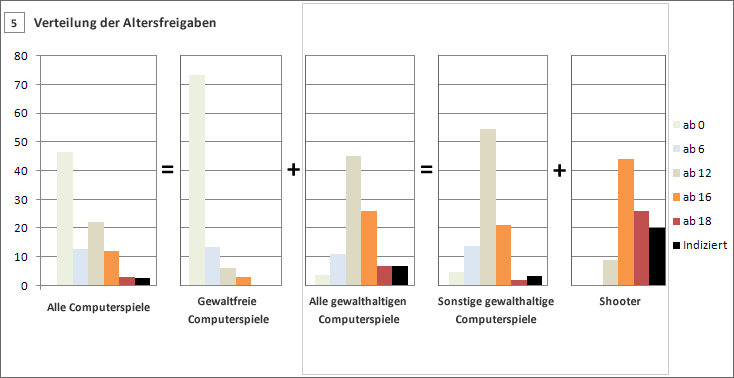
\includegraphics[width=0.8\textwidth]{images/stigmafreigaben}
\caption[Statistik der USK-Altersfreigaben nach Genres seit 1994]{Statistik der USK-Altersfreigaben nach Genres seit 1994\footnotemark}
\label{figure:stigmafreigaben}
\end{figure}
\footnotetext{Quelle: http://stigma-videospiele.de/wordpress/rechtslage/statistiken/}

\section{Zielsetzung}
Ziel dieser Arbeit ist die Analyse des Genres Multiplayer-Taktik-Shooter und die Erarbeitung eines Konzepts f�r einen
gewaltfreien Genrevertreter. Es soll gezeigt werden, dass das Spielprinzip des Shooters auch ohne Gewaltdarstellungen,
speziell ohne Schie�en auf und T�ten von Gegnern, funktioniert. Dazu sollen zum Einen die Eigenschaften, in denen sich
der Shooter au�er dem Schie�en noch von anderen Genres unterscheidet und damit selbst definiert, identifiziert und
verwendet werden. Zum Anderen sollen M�glichkeiten f�r neue Spielelemente gefunden und untersucht werden, die eine
eventuell entstehende L�cke im Konzept durch den Wegfall des Elements "`Schie�en"' f�llen oder ausgleichen k�nnen.\\

Es soll also eine M�glichkeit aufgezeigt werden, ein gutes Spiel zu entwickeln, das alle Eigenschaften und Elemente des
Shooters hat, die mit dem gewaltfreien Grundsatz vereinbar sind und somit das gleiche Klientel zufriedenstellt.

\begin{center}
Shooter - Schie�en + X $\rightarrow$ Spielqualit�t
\end{center}

Dabei ist mit Spielqualit�t Spielspa�, Motivation und Schwierigkeit gemeint, die an den Erwartungen von Shooterspielern
gemessen werden. Der Platzhalter X steht f�r Spielemente, die neu hinzugef�gt werden. Solche sollen in dieser Arbeit
gefunden und erprobt werden.

\chapter{Theoretischer Hintergrund}
\label{chapter:Background}

\section{Spielspa�}

Um zu verstehen, was ein gutes Computerspiel ausmacht, muss zuerst untersucht werden, warum sie �berhaupt genutzt
werden. Dazu wird im Folgenden ein kurzer �berblick �ber die derzeitige wissenschaftliche Meinung gegeben werden.

\subsection{Motivation}
Die am h�ufigsten genannten Situationen, aus denen der Wunsch, zum Computerspiel zu greifen, entsteht, sind Langeweile
(Wunsch nach Unterhaltung), Stress (Wunsch nach Stressabbau), �rger oder Wut (Wunsch nach Aggressionsabbau) und soziale
Motive (zum Spielen verabredet). \cite[S. 93]{Ladas_2002}\cite[S. 65ff]{Koehler_2008} Die Spieler erwarten von der
Nutzung des Spiels also eine Ablenkung von ihrer realen Situation, etwas Spannendes zu erleben, und sich dadurch nachher
besser zu f�hlen als davor. \cite[S. 66]{Koehler_2008}  Spieler w�hlen zu diesem Zweck vor allem Spiele, die eine
gewisse Verbindung zu ihrem Leben haben. Faktoren, die dabei eine Rolle spielen, sind laut \cite[S. 95]{Ladas_2002}:
\begin{itemize}
\item Assoziationen zu fr�heren Kinderspielen
\item Hobbys
\item Filmvorlieben
\item Wunsch nach Abenteuer, Erlebnissen
\item Ablehnung von Gewalt und Krieg
\item Ausleben von Ordnungssinn/�hnlichkeiten zur Organisation des 'realen' Lebens
\item Erinnerungen an bestimmte Lebenssituationen (belastend oder positiv)
\end{itemize}
Zur Motivation geh�rt aber auch der Wunsch nach Macht, Kontrolle, Leistung, Kompetenz und Erfolg: 
\begin{quotation}
Aufgrund dieses Wunsches ist der Spieler immer wieder motiviert, sich mit dem Spiel zu besch�ftigen. Das Entwickeln erfolgreicher Schemata, das Unter-Kontrolle-Bringen von Situationen, das Erledigen von Aufgaben, Zeigen von Leistung, Erwerb von Kompetenz, um Kontrolle und Macht zu erlangen und erfolgreich zu sein, sind sowohl Merkmale von Computerspielen als auch vom realen Leben. \cite[S. 74]{Koehler_2008}
\end{quotation}

\subsection{Interaktivit�t}
Computerspiele unterscheiden sich von anderen audiovisuellen Medien vor allem durch eine unabdingbare Notwendigkeit der
Steuerung durch den Benutzer. \cite[59]{Ladas_2002} Diese Interaktivit�t sehen die meisten Forscher als zentrale
Komponente des Unterhaltungserlebens der Spieler an. \cite{Klimmt_2006} Wesentlich dabei ist die direkte Reaktion auf
jede Eingabe des Spielers. Die Wichtigkeit direkten Feedbacks auf Benutzereingaben betont auch die Firma Apple, die von
vielen als Vorreiter in Sachen Benutzerschnittstellen bezeichnet wird, in ihrer "`iOS human interface guidelines"'.
\cite[20]{Apple_2012} Die direkte Reaktion auf Eingaben, in Spielen meist in Form einer Ver�nderung innerhalb der
virtuellen Umgebung, gibt dem Spieler das Gef�hl, etwas zu bewirken. Die Motivationspsychologie stellt den Begriff
"`effectance"' \cite{White_1959}, der den positiven emotionalen Einfluss von Selbswirksamkeitserfahrungen beschreibt.
Computerspiele verursachen starke Effectance-Erfahrungen, indem sie den Spieler meist die Spielwelt mit wenigen Eingaben
wesentlich ver�ndern lassen. \cite{Klimmt_2006_Effectance} Da Computerspiele stets verl�sslich direkte Reaktionen auf
Eingaben des Spielers geben, rufen sie bei Spielern kontinuierlich Effectance-Erfahrungen hervor. \cite{Klimmt_2006}
Selbstwirksamkeitserfahrungen erleben die Spieler folglich des interaktiven Charakters von Computerspielen, weshalb
dieser als wesentlicher Aspekt des Spielspa�es betrachtet werden muss.

\subsection{Leistungshandeln}
Spiele verlangen vom Spieler meist, ein schwieriges Problem zu l�sen oder Aufgaben zu bew�ltigen. \cite{Oerter_1999} Bei
Multiplayer-Computerspielen kann beides gleichzeitig gefordert sein, wenn als Aufgabe das Erf�llen des Spielziels und
als Problem das dem eigenen entgegenstehende Spielziel des Gegners - und somit letztlich der Gegner an sich - gesehen
wird. Der Spieler muss also etwas leisten:
\begin{quotation}
Computerspiele fordern (dauerhaft) gute Leistungen und sie belohnen Leistungen mit verschiedenen Varianten von Belohnungen,[\ldots]. Sie bestrafen unzureichende Leistungen aber auch mit frustrierenden Erfahrungen. \cite{Behr_2008}
\end{quotation}
Die eintretenden Erfolge und Misserfolge rufen spezifische emotionale Konsequenzen hervor.
Erfolge, die auf die eigene F�higkeit zur�ckgef�hrt werden, erzeugen zum Beispiel Zuversicht und das Gef�hl der
Kompetenz. \cite{Behr_2008} Der Spieler wird also stets versucht sein, Erfolge zu maximieren und das Eintreten von Misserfolgen zu verhindern.

\section{Gewalt in Spielen}


\subsection{Historie}
Die ersten Spiele, in denen man auf virtuelle Gegner schie�en konnte, waren sog. Shot'em'Ups, Spiele in 2D-Grafik, bei
denen der Spieler Gegnerwellen, die langsam auf ihn zukommen, abschie�en muss. Besonders Space Invaders aus dem Jahr
1978 erreichte gro�e Beliebtheit. Gewaltdarstellungen waren zu dieser Zeit noch sehr abstrakt. So l�sten sich zum
Beispiel getroffene Alien-Angreifer lediglich mit einer kleinen flimmernden Pixel-Wolke in Luft auf.

Der erste First-Person-Shooter im heutigen Sinne wurde 1973 von dem Studenten Steve Colley entwickelt. In Maze War
konnte man sich bereits in einer 3D-Welt bewegen und auf Gegner schie�en, sowie �ber ein Netzwerk mit ca. 30 Spielern
zusammen spielen. Dennoch war es so gut wie gewaltfrei: Treffer wurden durch blinken des Bildschirms (oder Teilen davon)
erkenntlich gemacht, getroffene Spieler wurden lediglich an eine zuf�llige Position bef�rdert und konnten von dort aus
weiterspielen.

Ein weiterer Meilenstein in der Entwicklung von Computerspielen und gleichzeitig ein erstes negatives Extrem im Bezug
auf Gewaltdarstellungen war Wolfenstein 3D, das 1992 von id Software ver�ffentlicht wurde. Wolfenstein 3D wurde von der
Bundespr�fstelle f�r jugendgef�hrdende Schriften 1994 aufgrund der sehr realistischen Darstellung der T�tung
menschlicher Gegner, sowie, weil der Spieler gezwungen war, massenhaft menschliche Gegner zu t�ten, um selbst zu
�berleben, indiziert. \\

\begin{figure}[h]
\centering
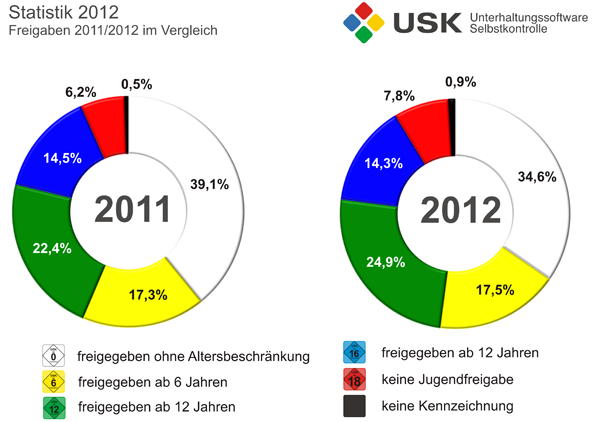
\includegraphics[width=0.8\textwidth]{images/uskfreigaben2012}
\caption[http://www.usk.de/pruefverfahren/statistik/]{Statistik der USK}
\label{uskfreigaben2012}
\end{figure}

Die Statistik der USK zeigt, dass heute ebenfalls viele Spiele f�r Jugendliche ungeeignete Darstellungen von
Gewalt enthalten. 2012 erhielten 8,7 Prozent der gepr�ften Spiele keine Freigabe f�r Jugendliche.


\subsection{Altersfreigaben}
Spiele, die Gewalt (meist in Form von Kampfhandlungen) enthalten, gibt es gleicherma�en in den USK-Alterseinteilungen
"ab 12", "ab 16", "keine Jugendfreigabe" sowie bei Spielen, f�r die die USK die Kennzeichnung verweigerte (Siegel "keine
Kennzeichnung"). Den Unterschied zwischen den ersten drei Stufen macht vor allem der Realit�tsgrad, die
�bertragbarkeitauf die Realit�t und den Alltag, sowie der auf den Spieler ausge�bte Druck, gewaltt�tige Handlungen zu
vollziehen, aus. Das Siegel "Keine Kennzeichnung", das fast immer eine Indizierung durch die BPjM nach sich zieht,
bedeutet dagegen,

\begin{itemize} 
  \item dass Spielinhalte Gewalttaten in der Alltagswirklichkeit legitimieren und Parallelen zur Realit�t nahelegen;
  \item dass das Spiel nur erfolgreich beendet werden kann, wenn Spielfiguren eliminiert werden, die nicht als Gegner auftreten;
  \item dass drastisch inszenierte und grafisch detailliert aufbereitete Gewalttaten gegen menschlich oder menschen�hnlich gestaltete Spielfiguren die Spielhandlung pr�gen;
  \item dass Kriegsbegeisterung vermittelt und Gewaltfolgen explizit bagatellisiert werden.\cite{uskalterskennzeichen}
\end{itemize} 

Das bedeutet, dass Gewalt in Spielen, zumindest laut der Einsch�tzung der Bundespr�fstelle f�r jugendgef�hrdende Medien
(BPjM), nicht zwingend jugendgef�hrdend sein muss, dies aber je nach Darstellung und Rahmenbedingungen sein kann.

\subsection{Gr�nde}
Man k�nnte annehmen, das h�ufige Auftreten von Gewaltdarstellungen in Spielen w�re historisch bedingt. Forschungen im
Bereich der Computertechnik wurden von Beginn an vom Milit�r forciert und finanziert. Das legt nahe, dass milit�rische
Simulationen die Inspiration zu den ersten Computerspielen waren, woraufhin sich der Bezug zur Gewalt einfach bis heute
erhalten haben k�nnte. Die Geschichte spricht jedoch dagegen, wie weiter oben bereits dargestellt. Der erste Shooter der
Welt war gewaltfrei und entwickelt von einem Studenten. Die andauernde Pr�senz von Gewalt in Computerspielen muss als
einen anderen Grund haben.\\

Kunczik und Zipfel haben die verschiedenen Erkl�rungsans�tze dazu gesammelt:
\itemize{begin}
\item 1. �sthetische Funktionen Hierbei wird den Gewaltdarstellungen eine
�sthetische Funktion unterstellt. Gewaltszenen sollen unabh�ngig vom Kontext
durch Ger�usche, Bewegungen, Farben usw. als angenehme Sinneseindr�cke
wahrgenommen werden.
\item 2. Evolutionstheoretischer Ansatz Diesem Ansatz zufolge ist der Reiz des
Neuen und Ungew�hnlichen verantwortlich f�r die Attraktivit�t der Mediengewalt.
Die Rede ist hier vo einer "morbiden Neugierde", die von Gefahr, Verletzung und
Tod ausgehe. Auch Voyeurismus sowie die im Alltagsleben f�r gew�hnlich nicht zu
beobachtende Verletzung sozialer Normen k�nnen ein Zuschauermotiv sein.
\item 3. Mood-Management Die Mood-Management-Theorie besagt, dass die Auswahl
und Nutzung von Medieninhalten der Stimmungsregulierung dient. Gewalthaltige
Medien k�nnen dieser Theorie zufolge attraktiv sein, weil sie ein zu greinges
Erregungsniveu anheben.
\item 4. Excitation-Transfer Laut der Excistation-Transfer-Theorie verst�rken
Erregungszust�nde auch die Intensit�t von Gef�hlen, die mit dem
erregungsausl�senden Stimulus nicht verbunden sind. "Ein Zustand erh�hter
Erregung, der aus furchteinfl��enden Medieninhalten resultiert, kann dazu
f�hren, dass auch die Erleichterung �ber einen guten Ausgang der
angstausl�senden Handlung intensiver wahrgenommen wird." \item 5.
Dispositionstheorie Die Dispositionstheorie basiert auf der Annahme, dass
Rezipienten auf Mediendarstellungen genauso reagieren, wie auf Ereignisse in der
Realit�t. So bilde der Zuschauer bei der Beobachtung von Geschehnissen
Sympathien und Antipathien f�r die Protagonisten aus. Leiden unsympathische
Protagonisten unter Gewalt, empfinde der Zuschauer diese als gerechte
Bestrafung, und k�nne sie daher genie�en.
\item 6. Sensation-Seeking Nach der Sensation-Seeking-Theorie suchen manche
Menschen stets nach neuen, intensiveren Reizen und Erfahrungen. Der Konsum
violenter Medieninhalte k�nne zum Erreichen des (bei diesen Menschen h�heren)
optimalen Erregungsniveaus beitragen, und somit gratifizierend wirken.
\item 7. Gruppenzugeh�rigkeit und Identit�tsbildung Eine weitere Motivation
gewalthaltige Medien zu konsumieren, kann (vor allem f�r Jugendliche) der Wunsch
nach Gruppenzugeh�rigkeit sein, die Medieninhalte werden also genutzt, um
mitreden zu k�nnen, sowie, um Mut zu beweisen. In diesem Zusammenhang kann auch
die Rolle von gewalthaltigen Medien in der Entwicklung von Jugendlichen gesehen
werden, wo sie sowohl als Abgrenzung gegen�ber den Erwachsenen (Eltern und
Lehrer) als auch gegen�ber der Kindheit und somit, in Anlehnung an
Initiationsriten alter Zeiten, als �bergang zum Erwachsenenalter, dient.
\item 8. Angstbew�ltigung und Angstlust Diese Theorie erkl�rt die
angstreduzierende Wirkung der Nutzung gewalthaltiger Medien durch Stimulation
der Angst verarbeitenden und kontrollierenden Mechanismen. Aber auch ohne diesen
trainierenden Effekt kann Angst als Motiv gesehen werden, n�mlich dann, wenn der
Zuschauer aufgrund seiner sicheren Situation Angst oder Furcht lustvoll
druchleben kann.
\item 9. Aggressive Pr�disposition Aggressive Pr�dispositionen von Rezipienten k�nnen ebenfalls
zur Begr�ndung f�r die Wahl gewalthaltiger Medieninhalte herangezogen werden. Der
kausale Zusammenhang von Aggresivit�t und Mediengewalt gilt als best�tigt,
wenngleich die Wirkrichtung bisher nicht gekl�rt werden konnte. 
\cite{kunczik}

\subsection{Wirkung}
�ber die Wirkung von Gewaltdarstellungen in Computerspielen bzw. in Medien allgemein gehen die Meinungen stark auseinander.

\chapter{Multiplayer-Taktik-Shooter}
\label{chapter:multiplayerTacticShooter}

\section{Definition und Abgrenzung}
Heutige Computerspiele werden h�ufig einem der folgenden Genres zugesprochen: Shooter, Strategie, Rollenspiele. Diese
Liste ist nat�rlich weder vollst�ndig, noch ist die Zuordnung stets eindeutig. Alle Genres haben diverse Subgenres, es
gibt Spiele, die Elemente aus mehreren Genres vereinen, sog. Hybride. Au�erdem kann in fast jedem Genre noch nach
Singleplayer, Multiplayer oder Massive-Multiplayer unterschieden werden.\\

Um f�r die vorliegende Arbeit Unklarheiten und Missverst�ndnisse so gut es get zu vermeiden, soll im folgenden das
Subgenre der Multiplayer-Taktik-Shooter definiert und zu anderen Genres abgegrenzt werden. Die Definition l�sst sich
leicht anhand der einzelnen Namensbestandteile erl�utern.

\subsubsection{Shooter}
Ein Shooter ist ein Spiel, bei dem der Spieler einen einzelnen Avatar in einer virtuellen Welt steuert. Die
Steuerung erfolgt klassisch �ber Maus und Tastatur, wobei die Maus zum Umsehen und Zielen, die Maustasten zum Feuern der
Waffe und die Tastatur zum Bewegen benutzt wird. Das Spielziel ist meist das T�ten des Gegners mit einer Waffe.
Existiert ein alternatives Spielziel, so ist das Ausschalten des Gegners n�tig oder zumindest zutr�glich f�r das
Erreichen desselben.\\

Eine weitere Unterscheidung l�sst sich anhand der Perspektive feststellen. Von den drei
M�glichkeiten first-person, third-person und top-down ist erstere die bei Shootern am h�ufigsten eingesetzte. Auch
in der vorliegenden Arbeit soll diese verwendet werden.

\subsubsection{Taktik}
W�hrend in einem reinen Ego-Shooter der Spielablauf ausschlie�lich darauf ausgerichtet ist, Gegner zu t�ten und dabei
kein besonderes taktisches Vorgehen verlangt ist, sind in einem Taktik-Shooter unter anderem Fahigkeiten wie geschickte
Positionierung, Timing, Kenntnis der Umgebung, Abstimmung im Team gefordert. Das Schie�en auf den Gegner und die dabei
geforderte Pr�zision sind somit nicht allein spielentscheidend.

\subsubsection{Multiplayer}
Als Multiplayer-Spiel bezeichnet man ein Computerspiel, das �ber Netzwerk oder Internet von mehreren Spielern gemeinsam
gespielt wird. Die Avatare der Spieler befinden sich in einer gemeinsamen virtuellen Welt. Diese Welt wird von der
Spielmechanik so synchronisiert, dass alle Spieler Ereignisse und Ver�nderungen darin in gleicher Weise wahrnehmen
k�nnen. Gegner und Teammitglieder werden teilweise oder ausschlie�lich von realen Mitspielern gesteuert, was trotz der
stetig voranschreitenden KI-Entwicklung auch heute noch ein dynamischeres und realistischeres Verhalten der virtuellen
Spielfiguren erzeugt als bei sog. "BOTs" (engl. kurz f�r "robot"), vom Computer simulierten Mitspielern. 

\subsection{Weitere Abgrenzung}
Das Spiel l�uft in Runden mit stets der gleichen Ausgangssituation ab. Auf eine Handlung im Sinne eines Drehbuchs (wie
bei Singleplayer-Spielen �blich) sowie auf eine fortgesetzte Entwicklung der Spielwelt sowie des Charakters/Avatars (wie
bei Singleplayer- und Rollenspielen �blich) wird weitestgehend verzichtet.\\

Die Spielerzahl liegt in einem �berschaubaren Bereich. �blicherweise zwischen 10 und 64 Spielern pro Instanz, aber auch
Spiele mit bis zu 128 oder gar noch mehr Spielern sind bereits zu finden. Dennoch deutlich ist der Unterschied zu sog.
MMOs, bei denen oft mehrere tausend Spieler in einer Instanz spielen.\\

Bekannte Multiplayer-Taktik-Shooter im Sinne dieser Definition sind z.B. Counterstrike, Battlefield und Call of Duty.
Nicht darunter fallen Singleplayer-Spiele wie Tomb Raider und Splinter-Cell oder Shooter, denen der Taktik-Anteil fehlt,
wie z.B. Quake 3 Arena.\\
%\section{Gewalt in Spielen}


\subsection{Historie}
Die ersten Spiele, in denen man auf virtuelle Gegner schie�en konnte, waren sog. Shot'em'Ups, Spiele in 2D-Grafik, bei
denen der Spieler Gegnerwellen, die langsam auf ihn zukommen, abschie�en muss. Besonders Space Invaders aus dem Jahr
1978 erreichte gro�e Beliebtheit. Gewaltdarstellungen waren zu dieser Zeit noch sehr abstrakt. So l�sten sich zum
Beispiel getroffene Alien-Angreifer lediglich mit einer kleinen flimmernden Pixel-Wolke in Luft auf.

Der erste First-Person-Shooter im heutigen Sinne wurde 1973 von dem Studenten Steve Colley entwickelt. In Maze War
konnte man sich bereits in einer 3D-Welt bewegen und auf Gegner schie�en, sowie �ber ein Netzwerk mit ca. 30 Spielern
zusammen spielen. Dennoch war es so gut wie gewaltfrei: Treffer wurden durch blinken des Bildschirms (oder Teilen davon)
erkenntlich gemacht, getroffene Spieler wurden lediglich an eine zuf�llige Position bef�rdert und konnten von dort aus
weiterspielen.

Ein weiterer Meilenstein in der Entwicklung von Computerspielen und gleichzeitig ein erstes negatives Extrem im Bezug
auf Gewaltdarstellungen war Wolfenstein 3D, das 1992 von id Software ver�ffentlicht wurde. Wolfenstein 3D wurde von der
Bundespr�fstelle f�r jugendgef�hrdende Schriften 1994 aufgrund der sehr realistischen Darstellung der T�tung
menschlicher Gegner, sowie, weil der Spieler gezwungen war, massenhaft menschliche Gegner zu t�ten, um selbst zu
�berleben, indiziert. \\

\begin{figure}[h]
\centering
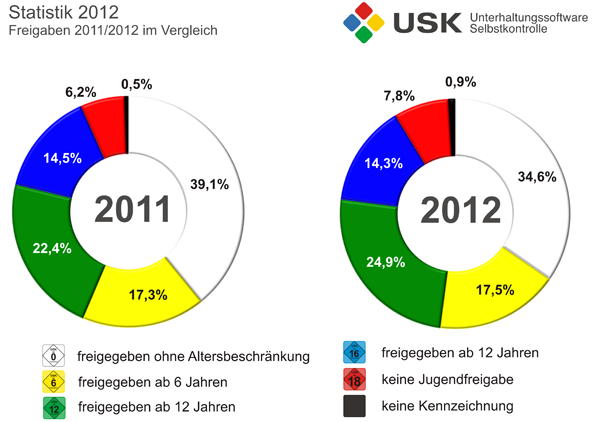
\includegraphics[width=0.8\textwidth]{images/uskfreigaben2012}
\caption[http://www.usk.de/pruefverfahren/statistik/]{Statistik der USK}
\label{uskfreigaben2012}
\end{figure}

Die Statistik der USK zeigt, dass heute ebenfalls viele Spiele f�r Jugendliche ungeeignete Darstellungen von
Gewalt enthalten. 2012 erhielten 8,7 Prozent der gepr�ften Spiele keine Freigabe f�r Jugendliche.


\subsection{Altersfreigaben}
Spiele, die Gewalt (meist in Form von Kampfhandlungen) enthalten, gibt es gleicherma�en in den USK-Alterseinteilungen
"ab 12", "ab 16", "keine Jugendfreigabe" sowie bei Spielen, f�r die die USK die Kennzeichnung verweigerte (Siegel "keine
Kennzeichnung"). Den Unterschied zwischen den ersten drei Stufen macht vor allem der Realit�tsgrad, die
�bertragbarkeitauf die Realit�t und den Alltag, sowie der auf den Spieler ausge�bte Druck, gewaltt�tige Handlungen zu
vollziehen, aus. Das Siegel "Keine Kennzeichnung", das fast immer eine Indizierung durch die BPjM nach sich zieht,
bedeutet dagegen,

\begin{itemize} 
  \item dass Spielinhalte Gewalttaten in der Alltagswirklichkeit legitimieren und Parallelen zur Realit�t nahelegen;
  \item dass das Spiel nur erfolgreich beendet werden kann, wenn Spielfiguren eliminiert werden, die nicht als Gegner auftreten;
  \item dass drastisch inszenierte und grafisch detailliert aufbereitete Gewalttaten gegen menschlich oder menschen�hnlich gestaltete Spielfiguren die Spielhandlung pr�gen;
  \item dass Kriegsbegeisterung vermittelt und Gewaltfolgen explizit bagatellisiert werden.\cite{uskalterskennzeichen}
\end{itemize} 

Das bedeutet, dass Gewalt in Spielen, zumindest laut der Einsch�tzung der Bundespr�fstelle f�r jugendgef�hrdende Medien
(BPjM), nicht zwingend jugendgef�hrdend sein muss, dies aber je nach Darstellung und Rahmenbedingungen sein kann.

\subsection{Gr�nde}
Man k�nnte annehmen, das h�ufige Auftreten von Gewaltdarstellungen in Spielen w�re historisch bedingt. Forschungen im
Bereich der Computertechnik wurden von Beginn an vom Milit�r forciert und finanziert. Das legt nahe, dass milit�rische
Simulationen die Inspiration zu den ersten Computerspielen waren, woraufhin sich der Bezug zur Gewalt einfach bis heute
erhalten haben k�nnte. Die Geschichte spricht jedoch dagegen, wie weiter oben bereits dargestellt. Der erste Shooter der
Welt war gewaltfrei und entwickelt von einem Studenten. Die andauernde Pr�senz von Gewalt in Computerspielen muss als
einen anderen Grund haben.\\

Kunczik und Zipfel haben die verschiedenen Erkl�rungsans�tze dazu gesammelt:
\itemize{begin}
\item 1. �sthetische Funktionen Hierbei wird den Gewaltdarstellungen eine
�sthetische Funktion unterstellt. Gewaltszenen sollen unabh�ngig vom Kontext
durch Ger�usche, Bewegungen, Farben usw. als angenehme Sinneseindr�cke
wahrgenommen werden.
\item 2. Evolutionstheoretischer Ansatz Diesem Ansatz zufolge ist der Reiz des
Neuen und Ungew�hnlichen verantwortlich f�r die Attraktivit�t der Mediengewalt.
Die Rede ist hier vo einer "morbiden Neugierde", die von Gefahr, Verletzung und
Tod ausgehe. Auch Voyeurismus sowie die im Alltagsleben f�r gew�hnlich nicht zu
beobachtende Verletzung sozialer Normen k�nnen ein Zuschauermotiv sein.
\item 3. Mood-Management Die Mood-Management-Theorie besagt, dass die Auswahl
und Nutzung von Medieninhalten der Stimmungsregulierung dient. Gewalthaltige
Medien k�nnen dieser Theorie zufolge attraktiv sein, weil sie ein zu greinges
Erregungsniveu anheben.
\item 4. Excitation-Transfer Laut der Excistation-Transfer-Theorie verst�rken
Erregungszust�nde auch die Intensit�t von Gef�hlen, die mit dem
erregungsausl�senden Stimulus nicht verbunden sind. "Ein Zustand erh�hter
Erregung, der aus furchteinfl��enden Medieninhalten resultiert, kann dazu
f�hren, dass auch die Erleichterung �ber einen guten Ausgang der
angstausl�senden Handlung intensiver wahrgenommen wird." \item 5.
Dispositionstheorie Die Dispositionstheorie basiert auf der Annahme, dass
Rezipienten auf Mediendarstellungen genauso reagieren, wie auf Ereignisse in der
Realit�t. So bilde der Zuschauer bei der Beobachtung von Geschehnissen
Sympathien und Antipathien f�r die Protagonisten aus. Leiden unsympathische
Protagonisten unter Gewalt, empfinde der Zuschauer diese als gerechte
Bestrafung, und k�nne sie daher genie�en.
\item 6. Sensation-Seeking Nach der Sensation-Seeking-Theorie suchen manche
Menschen stets nach neuen, intensiveren Reizen und Erfahrungen. Der Konsum
violenter Medieninhalte k�nne zum Erreichen des (bei diesen Menschen h�heren)
optimalen Erregungsniveaus beitragen, und somit gratifizierend wirken.
\item 7. Gruppenzugeh�rigkeit und Identit�tsbildung Eine weitere Motivation
gewalthaltige Medien zu konsumieren, kann (vor allem f�r Jugendliche) der Wunsch
nach Gruppenzugeh�rigkeit sein, die Medieninhalte werden also genutzt, um
mitreden zu k�nnen, sowie, um Mut zu beweisen. In diesem Zusammenhang kann auch
die Rolle von gewalthaltigen Medien in der Entwicklung von Jugendlichen gesehen
werden, wo sie sowohl als Abgrenzung gegen�ber den Erwachsenen (Eltern und
Lehrer) als auch gegen�ber der Kindheit und somit, in Anlehnung an
Initiationsriten alter Zeiten, als �bergang zum Erwachsenenalter, dient.
\item 8. Angstbew�ltigung und Angstlust Diese Theorie erkl�rt die
angstreduzierende Wirkung der Nutzung gewalthaltiger Medien durch Stimulation
der Angst verarbeitenden und kontrollierenden Mechanismen. Aber auch ohne diesen
trainierenden Effekt kann Angst als Motiv gesehen werden, n�mlich dann, wenn der
Zuschauer aufgrund seiner sicheren Situation Angst oder Furcht lustvoll
druchleben kann.
\item 9. Aggressive Pr�disposition Aggressive Pr�dispositionen von Rezipienten k�nnen ebenfalls
zur Begr�ndung f�r die Wahl gewalthaltiger Medieninhalte herangezogen werden. Der
kausale Zusammenhang von Aggresivit�t und Mediengewalt gilt als best�tigt,
wenngleich die Wirkrichtung bisher nicht gekl�rt werden konnte. 
\cite{kunczik}

\subsection{Wirkung}
�ber die Wirkung von Gewaltdarstellungen in Computerspielen bzw. in Medien allgemein gehen die Meinungen stark auseinander.

%\chapter{Multiplayer-Taktik-Shooter}
\label{chapter:multiplayerTacticShooter}

\section{Definition und Abgrenzung}
Heutige Computerspiele werden h�ufig einem der folgenden Genres zugesprochen: Shooter, Strategie, Rollenspiele. Diese
Liste ist nat�rlich weder vollst�ndig, noch ist die Zuordnung stets eindeutig. Alle Genres haben diverse Subgenres, es
gibt Spiele, die Elemente aus mehreren Genres vereinen, sog. Hybride. Au�erdem kann in fast jedem Genre noch nach
Singleplayer, Multiplayer oder Massive-Multiplayer unterschieden werden.\\

Um f�r die vorliegende Arbeit Unklarheiten und Missverst�ndnisse so gut es get zu vermeiden, soll im folgenden das
Subgenre der Multiplayer-Taktik-Shooter definiert und zu anderen Genres abgegrenzt werden. Die Definition l�sst sich
leicht anhand der einzelnen Namensbestandteile erl�utern.

\subsubsection{Shooter}
Ein Shooter ist ein Spiel, bei dem der Spieler einen einzelnen Avatar in einer virtuellen Welt steuert. Die
Steuerung erfolgt klassisch �ber Maus und Tastatur, wobei die Maus zum Umsehen und Zielen, die Maustasten zum Feuern der
Waffe und die Tastatur zum Bewegen benutzt wird. Das Spielziel ist meist das T�ten des Gegners mit einer Waffe.
Existiert ein alternatives Spielziel, so ist das Ausschalten des Gegners n�tig oder zumindest zutr�glich f�r das
Erreichen desselben.\\

Eine weitere Unterscheidung l�sst sich anhand der Perspektive feststellen. Von den drei
M�glichkeiten first-person, third-person und top-down ist erstere die bei Shootern am h�ufigsten eingesetzte. Auch
in der vorliegenden Arbeit soll diese verwendet werden.

\subsubsection{Taktik}
W�hrend in einem reinen Ego-Shooter der Spielablauf ausschlie�lich darauf ausgerichtet ist, Gegner zu t�ten und dabei
kein besonderes taktisches Vorgehen verlangt ist, sind in einem Taktik-Shooter unter anderem Fahigkeiten wie geschickte
Positionierung, Timing, Kenntnis der Umgebung, Abstimmung im Team gefordert. Das Schie�en auf den Gegner und die dabei
geforderte Pr�zision sind somit nicht allein spielentscheidend.

\subsubsection{Multiplayer}
Als Multiplayer-Spiel bezeichnet man ein Computerspiel, das �ber Netzwerk oder Internet von mehreren Spielern gemeinsam
gespielt wird. Die Avatare der Spieler befinden sich in einer gemeinsamen virtuellen Welt. Diese Welt wird von der
Spielmechanik so synchronisiert, dass alle Spieler Ereignisse und Ver�nderungen darin in gleicher Weise wahrnehmen
k�nnen. Gegner und Teammitglieder werden teilweise oder ausschlie�lich von realen Mitspielern gesteuert, was trotz der
stetig voranschreitenden KI-Entwicklung auch heute noch ein dynamischeres und realistischeres Verhalten der virtuellen
Spielfiguren erzeugt als bei sog. "BOTs" (engl. kurz f�r "robot"), vom Computer simulierten Mitspielern. 

\subsection{Weitere Abgrenzung}
Das Spiel l�uft in Runden mit stets der gleichen Ausgangssituation ab. Auf eine Handlung im Sinne eines Drehbuchs (wie
bei Singleplayer-Spielen �blich) sowie auf eine fortgesetzte Entwicklung der Spielwelt sowie des Charakters/Avatars (wie
bei Singleplayer- und Rollenspielen �blich) wird weitestgehend verzichtet.\\

Die Spielerzahl liegt in einem �berschaubaren Bereich. �blicherweise zwischen 10 und 64 Spielern pro Instanz, aber auch
Spiele mit bis zu 128 oder gar noch mehr Spielern sind bereits zu finden. Dennoch deutlich ist der Unterschied zu sog.
MMOs, bei denen oft mehrere tausend Spieler in einer Instanz spielen.\\

Bekannte Multiplayer-Taktik-Shooter im Sinne dieser Definition sind z.B. Counterstrike, Battlefield und Call of Duty.
Nicht darunter fallen Singleplayer-Spiele wie Tomb Raider und Splinter-Cell oder Shooter, denen der Taktik-Anteil fehlt,
wie z.B. Quake 3 Arena.\\


%
%% ---------------------------------------------------------------------------
%%
%% Gewaltfreier Shooter
%%
%%% ---------------------------------------------------------------------------
%\part[Gewaltfreies Computerspiel]{Gewaltfreies Computerspiel}
%\label{part:nonviolentComputerGame}
\chapter{High Concept}
\label{chapter:HighConcept}

\section{Szenarien}

Ein Szenario ist die konkrete, fokussierte und informelle Beschreibung eines einzelnen Systemmerkmals aus der Sichtweise
eines einzelnen Benuzters.\cite[S. 157]{BrueggeDutoit}

\subsection{Szenario 1: Server starten}
Peter startet das Spiel auf seinem Computer und aktiviert die Funktion "`Server starten"'. Anschlie�end w�hlt er die
Karte aus, auf der die Spieler auf seinem Server spielen sollen, und aktiviert die Funktion "`Karte laden"'. 

\subsection{Szenario 2: Spiel beitreten}
Hans m�chte auf dem Server von Peter, der sich im gleichen lokalen Netzwerk befindet, spielen. Dazu startet er das
Spiel, w�hlt den Server von Peter aus und nutzt die Funktion "`Mit Server verbinden"'. Er w�hlt Team 1 aus und beginnt zu spielen.

\subsection{Szenario 3: Connect via IP}
Auf einen Server connecten, der nicht in der Liste erscheint.????????????????????????????????????????????????

\subsection{Szenario 4: Karte wechseln}
Peter m�chte, dass ab sofort auf seinem Server auf einer anderen Karte gespielt wird. Dazu w�hlt er die neue Karte aus und aktiviert die Funktion "`Karte laden"'.
\section{Anwendungsfall-Modell}

"`Ein Anwendungsfall ist eine Abstraktion, die alle m�glichen Szenarien beschreiibt, die die beschriebene Funktionalit�t enthalten."'\cite[S. 76]{Bruegge_2004}\\
% Ein Szenario ist eine Instanz eines Anwendungsfalls; wenn wir diesen Anwendungsfall identifizieren, haben wir damit
% alle m�glichen Szenarien f�r eine gegebene Funktionalit�t.\cite[S. 160]{Bruegge_2004}

Anhand der in Abschnitt \ref{requirements} beschriebenen Anforderungen wurden die Anwendungsf�lle identifiziert, die
zeigen, wie die Anwendr mit dem System interagieren. In diesem Abschnitt wird das Anwendungsfall-Modell dargestellt und
die einzelnen Anwendungsf�lle erkl�rt. Ein vollst�ndiger Flow-of-Events zu jedem Anwendungsfall findet sich im Anhang.
Bei der Untersuchung der funktionellen Anforderungen wurden die Akteure Spieler und Administrator identifiziert.
Abbildung \ref{usecases} gibt einen �berblick �ber die Anwendungsf�lle aus Sicht von Spieler und Administrator.

\begin{figure}[htbp]
\centering
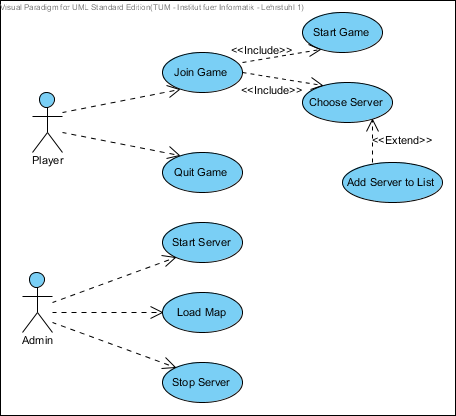
\includegraphics[width=0.8\textwidth]{images/usecases}
\caption[Anwendungsfall-Diagramm]{Anwendungsfall-Diagramm}
\label{usecases}
\end{figure}
\section{Anforderungen}
\label{requirements}


\section{Spielkonzept}

In diesem Kapitel soll anhand der bisher gewonnenen Erkenntnisse ein Spielkonzept erstellt werden, das den gewaltfreien
Ansatz verwirklicht und dabei die gew�nschten Shooter-Elemente enth�lt. Um Verwirrungen zu vermeiden, erh�lt das neue
Spiel bereits an dieser Stelle einen Namen, sozusagen einen Entwicklungs-Codenamen: Cydonia.


\subsection{Grundlegende Eigenschaften}
Cydonia soll ein Multiplayerspiel f�r ca. 5 bis 25 Spieler werden. Vorerst ist nur eine Unterst�tzung f�r
Local-Area-Network (LAN) n�tig, eine zuk�nftige Unterst�tzung von Spielen �ber das Internet ist jedoch nicht
auszuschlie�en.

Der Spieler soll seinen Avatar aus der Ego-Perspektive mittels Maus und Tastatur steuern k�nnen.

Cydonia bekommt ein futuristisches Setting, d.h. die Spielwelt sowie die Charaktere sind nicht der realen Gegenwart oder
Vergangenheit entnommen, sondern in einer fiktiven Zukunft angesiedelt. Dadurch wird zum einen die Schwierigkeit
umgangen, reale Lebewesen und Gegenst�nde �berzeugend und nat�rlich abzubilden, zum anderen bietet ein fiktives Setting
mehr kreativen Freiraum als ein reales, da unwahrscheinliche oder unm�gliche Dinge, Vorg�nge und Zusammenh�nge auf den
Spieler weniger irritierend wirken, wenn die gesamte Spielwelt bereits unrealistisch anmutet.


\subsection{Spielwelt}
Die virtuelle Welt von Cydonia besteht fast ausschlie�lich aus farbigen W�rfeln mit einem Meter Kantenl�nge. Diese
W�rfel bilden B�den, W�nde und D�cher. Die Spieler k�nnen eine W�rfelh�he �berspringen, wodurch auch Treppen m�glich
werden. Zur besseren semantischen Unterscheidung dieser W�rfel von der geometrischen Form werden die W�rfel der
Spielwelt im Folgenden "`Cube"' genannt.

\subsection{Spielmodus}
Cydonia bedient sich bei einem bekannten Modus, den bereits einige andere Shooter (z.B. Unreal Tournament) anbieten:
"`Capture the Flag"'. Dabei versuchen zwei Teams von Spielern, eine Flagge aus der gegnerischen in die eigene Basis zu
bringen und gleichzeitig das gegnerische Team von der eigenen Flagge fernzuhalten.


\subsection{Swapper}
Ein Equipment\footnote{vlg. dazu \ref{chapter:CaseStudy}} soll in Cydonia die Funktion der Waffen in anderen Shootern
�bernehmen, dem Spieler also eine direkte Einwirkung auf den Gegner erm�glichen. Mit dem sog. "`Swapper"' kann der
Spieler Cubes und andere Spieler markieren. Sobald er zwei Dinge markiert hat, tauschen diese beiden den Platz.
Dadurch kann der Spieler also seine Gegner von ihrem Pfad abbringen und in der Erf�llung ihres Auftrags behindern.
Gleichzeitig bietet sich aber auch die M�glichkeit, durch geschicktes "`Swappen"' von Mitgliedern des eigenen Teams
kooperativ zu agieren. Eine dritte Art der Verwendung besteht darin, durch das Vertauschen von Teilen der Spielwelt das
Leveldesign zum eigenen Vorteil zu ver�ndern. Bei der Benutzung sind genaues Zielen und gutes Timing n�tig, was die
gew�nschte haptische �hnlichkeit zu den typischen Waffen in Shootern ergibt. Au�erdem ist es erforderlich, taktisch und
vorausplanend mit den beiden verf�gbaren Markern umzugehen, worin sich eine Analogie zum Haushalten mit Munition im
Shooter finden l�sst. Die Aktion, zwei Objekte zu markieren sodass diese die Pl�tze tauschen, wird im Folgenden als
"`swappen"' bezeichnet.


\subsection{Pick'n'Place}
Der Spieler bekommt in Cydonia zudem ein Equipment in die Hand, das nicht auf Gegner, sondern ausschlie�lich auf Cubes
angewendet werden kann. Er kann damit bestimmte einzelne Cubes in seiner Umgebung entfernen und (an anderer Stelle)
wieder einf�gen und so das Leveldesign w�hrend des Spiels beeinflussen. Cubes, die der Spieler bewegen kann,
unterscheiden sich optisch von anderen.


\subsection{Nahkampf}
F�r das in Abschnitt \ref{subsection:CloseCombat} erl�uterte Spielelement Nahkampf konnte bisher keine gewaltfreie
Alternative gefunden werden, weshalb Cydonia vorerst auf ein solches Element verzichten muss.

\chapter{Systementwurf}
\label{chapter:SystemDesign}

\section{Systemzerlegung}
Bei der Systemzerlegung wird das System, basierend auf dem Anwendungsfall- und dem Analysemodell, in kleinere
Bestandteile zerlegt. \cite[S. 257ff]{Bruegge_2004}\\ % Sinngem��, kein w�rtliches Zitat.

Das System von Cydonia wurde in folgende Pakete zerlegt: Player, Equipment, GameWorld, GameController, Input.
Die Pakete Player und Equipment enthalten jeweils die zur Abbildung und Berechnung der Spieler bzw. der verschiedenen
Equipments ben�tigten Klassen.\\

Das Paket GameWorld fasst alle Klassen zusammen, die f�r die Generierung, Komposition, Simulation und Darstellung der
Spielwelt verantwortlich sind. Dazu geh�ren die Entit�ten f�r die Weltobjekte (Cube, Flagge, Spawnpunkt) sowie
Kontrollklassen, Fabriken und Schnittstellen.\\

Das Paket Input enth�lt die Klassen zur Verarbeitung von Benutzereingaben. Unter anderem werden darin variable
Tastenbelegungen und die Erzeugung von Steuerbefehlen implementiert.\\

Im Paket GameController befinden sich schlie�lich alle Klassen, die zur Initialisierung des Systems, Verwaltung von
Programmzust�nden und Steuerung von Men�s ben�tigt werden. Au�erdem wird hier auch die Logik, also der eigentliche
Ablauf, des Spiels umgesetzt.\\

Eine �bersicht �ber die Paketstruktur von Cydonia gibt auch Abbildung \ref{figure:global_control_flow}.

\begin{figure}[htbp]
\centering
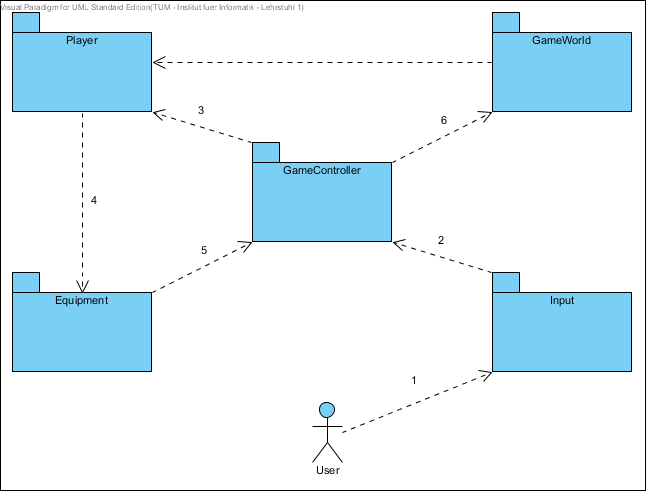
\includegraphics[width=1.0\textwidth]{images/global_control_flow}
\caption[UML-Paketdiagramm: Globaler Kontrollfluss]{UML-Paketdiagramm: Globaler Kontrollfluss}
\label{figure:global_control_flow}
\end{figure}

\section{Globaler Kontrollfluss}
\label{section:GlobalControlFlow}
Der f�r Computerspiele typische Kontrollfluss geht vom Spieler aus, der mit seinen Eingaben Ereignisse ausl�st.
Beispielsweise k�nnte der Spieler eine Taste dr�cken mit dem Ziel, einen Cube (mithilfe des Pick'n'Place-Equipments) in
der Spielwelt zu platzieren. Der Tastendruck wird vom Paket Input detektiert und in einen Steuerbefehl umgesetzt (z.B.
"`benutze equipment"'), welcher dann an das GameController-Paket weitergereicht wird. Dieses ermittelt die daraus
resultierende Reaktion, n�mlich dem Player-Paket den Befehl zu geben, das aktuelle Equipment des Spielers zu ermitteln
und dessen Benutzung anzusto�en, wodurch der Befehl im Equipment-Paket landet. Dort ist die auszuf�hrende Aktion f�r das
Pick'n'Place-Equipment implementiert (R�ckmeldungen f�r den Spieler, Manipulation der Spielwelt usw.).
Das Equipment-Paket meldet folglich dem GameController-Paket die gew�nschte Manipulation der Spielwelt, n�mlich das
Platzieren des im Equipment vorr�tigen Cubes an einer bestimmten Position. Letzendlich wird die Platzierung des Cubes im
Paket GameWorld ausgef�hrt und der Spieler kann den neuen Cube sehen. Dieser beispielhafte Ablauf kann auch anhand der
Nummerierung in Abbildung \ref{figure:global_control_flow} nachvollzogen werden.\\

Das Spiel hat jedoch auch Komponenten, die nicht ereignisgesteuert arbeiten. Das Rendern der virtuellen Welt sowie
deren physikalische Simulation laufen prozedural ab. In einer endlosen Schleife wird mehrmals pro Sekunde ein kleiner
Schritt des physikalischen Modells berechnet und ein neues Bild erzeugt.

\section{Hardware-Software Mapping}
Cydonia ist als Multiplayer-Spiel so konzipiert, dass mehrere Spieler zusammen in einer virtuellen Umgebung spielen.
Dabei nutzt jeder Spieler seinen eigenen Personal Computer (PC) (wie bei einem Singleplayer-Spiel) und die virtuelle
Welt wird zwischen den einzelnen Computern synchronisiert, damit alle Spieler den Lauf der Dinge konsistent erleben.
Dazu ist ein sog. Server n�tig, eine Instanz des Spiels, die die Autorit�t �ber die Geschehnisse in der virtuellen Welt
besitzt, da sonst durch geringf�gige Abweichungen in der Berechnung enorme Unterschiede zwischen den Simulationen auf
den einzelnen Computern entstehen k�nnen. Dieser Server kann bei ausreichender Rechenleistung auch auf einem der PCs der
Spieler laufen, der Einfachkeit halber soll im Folgenden jedoch nur der Fall eines dedizierten Servers betrachtet
werden. Abbildung \ref{figure:hardware_mapping} veranschaulicht die Verteilung der Software-Komponenten auf die
Hardware-Knoten.

\begin{figure}[htbp]
\centering
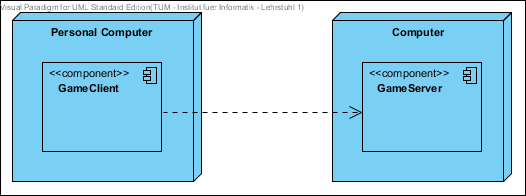
\includegraphics[width=0.8\textwidth]{images/hardware_mapping}
\caption[UML-Verteilungsdiagramm: Beziehung zwischen Software-Komponenten und Hardware-Knoten]{UML-Verteilungsdiagramm: Beziehung zwischen Software-Komponenten und Hardware-Knoten}
\label{figure:hardware_mapping}
\end{figure}

\section{Analyse Modell}


Cydonia stellt, wie viele Spiele, eine virtuelle Welt grafisch dar. Diese virtuelle Welt ist Teil der Anwendungsdom�ne
in der Spiele-Entwicklung. Somit finden sich die Elemente dieser Welt im Analyse-Modell wieder. Die Objekte des
Analyse-Modells wurden anhand der Anwendungsf�lle und Anforderungen identifiziert. Abbildung
\ref{figure:anlysis_classes} zeigt die w�hrend der Analyse identifizierten Objekte und ihre Beziehungen untereinander.

\begin{figure}[htbp]
\centering
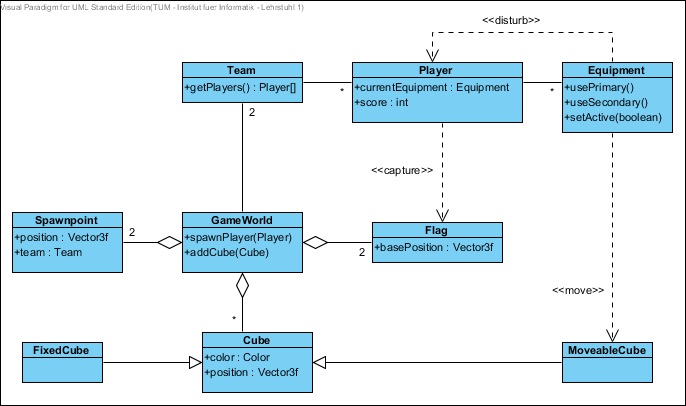
\includegraphics[width=0.8\textwidth]{images/analysis_class_diagramm}
\caption[UML-Klassendiagramm: Objekte der Anwendungsdom�ne]{UML-Klassendiagramm: Objekte der Anwendungsdom�ne}
\label{figure:anlysis_classes}
\end{figure}
%\section{Anforderungen}
\label{requirements}


%\section{Spielkonzept}

In diesem Kapitel soll anhand der bisher gewonnenen Erkenntnisse ein Spielkonzept erstellt werden, das den gewaltfreien
Ansatz verwirklicht und dabei die gew�nschten Shooter-Elemente enth�lt. Um Verwirrungen zu vermeiden, erh�lt das neue
Spiel bereits an dieser Stelle einen Namen, sozusagen einen Entwicklungs-Codenamen: Cydonia.


\subsection{Grundlegende Eigenschaften}
Cydonia soll ein Multiplayerspiel f�r ca. 5 bis 25 Spieler werden. Vorerst ist nur eine Unterst�tzung f�r
Local-Area-Network (LAN) n�tig, eine zuk�nftige Unterst�tzung von Spielen �ber das Internet ist jedoch nicht
auszuschlie�en.

Der Spieler soll seinen Avatar aus der Ego-Perspektive mittels Maus und Tastatur steuern k�nnen.

Cydonia bekommt ein futuristisches Setting, d.h. die Spielwelt sowie die Charaktere sind nicht der realen Gegenwart oder
Vergangenheit entnommen, sondern in einer fiktiven Zukunft angesiedelt. Dadurch wird zum einen die Schwierigkeit
umgangen, reale Lebewesen und Gegenst�nde �berzeugend und nat�rlich abzubilden, zum anderen bietet ein fiktives Setting
mehr kreativen Freiraum als ein reales, da unwahrscheinliche oder unm�gliche Dinge, Vorg�nge und Zusammenh�nge auf den
Spieler weniger irritierend wirken, wenn die gesamte Spielwelt bereits unrealistisch anmutet.


\subsection{Spielwelt}
Die virtuelle Welt von Cydonia besteht fast ausschlie�lich aus farbigen W�rfeln mit einem Meter Kantenl�nge. Diese
W�rfel bilden B�den, W�nde und D�cher. Die Spieler k�nnen eine W�rfelh�he �berspringen, wodurch auch Treppen m�glich
werden. Zur besseren semantischen Unterscheidung dieser W�rfel von der geometrischen Form werden die W�rfel der
Spielwelt im Folgenden "`Cube"' genannt.

\subsection{Spielmodus}
Cydonia bedient sich bei einem bekannten Modus, den bereits einige andere Shooter (z.B. Unreal Tournament) anbieten:
"`Capture the Flag"'. Dabei versuchen zwei Teams von Spielern, eine Flagge aus der gegnerischen in die eigene Basis zu
bringen und gleichzeitig das gegnerische Team von der eigenen Flagge fernzuhalten.


\subsection{Swapper}
Ein Equipment\footnote{vlg. dazu \ref{chapter:CaseStudy}} soll in Cydonia die Funktion der Waffen in anderen Shootern
�bernehmen, dem Spieler also eine direkte Einwirkung auf den Gegner erm�glichen. Mit dem sog. "`Swapper"' kann der
Spieler Cubes und andere Spieler markieren. Sobald er zwei Dinge markiert hat, tauschen diese beiden den Platz.
Dadurch kann der Spieler also seine Gegner von ihrem Pfad abbringen und in der Erf�llung ihres Auftrags behindern.
Gleichzeitig bietet sich aber auch die M�glichkeit, durch geschicktes "`Swappen"' von Mitgliedern des eigenen Teams
kooperativ zu agieren. Eine dritte Art der Verwendung besteht darin, durch das Vertauschen von Teilen der Spielwelt das
Leveldesign zum eigenen Vorteil zu ver�ndern. Bei der Benutzung sind genaues Zielen und gutes Timing n�tig, was die
gew�nschte haptische �hnlichkeit zu den typischen Waffen in Shootern ergibt. Au�erdem ist es erforderlich, taktisch und
vorausplanend mit den beiden verf�gbaren Markern umzugehen, worin sich eine Analogie zum Haushalten mit Munition im
Shooter finden l�sst. Die Aktion, zwei Objekte zu markieren sodass diese die Pl�tze tauschen, wird im Folgenden als
"`swappen"' bezeichnet.


\subsection{Pick'n'Place}
Der Spieler bekommt in Cydonia zudem ein Equipment in die Hand, das nicht auf Gegner, sondern ausschlie�lich auf Cubes
angewendet werden kann. Er kann damit bestimmte einzelne Cubes in seiner Umgebung entfernen und (an anderer Stelle)
wieder einf�gen und so das Leveldesign w�hrend des Spiels beeinflussen. Cubes, die der Spieler bewegen kann,
unterscheiden sich optisch von anderen.


\subsection{Nahkampf}
F�r das in Abschnitt \ref{subsection:CloseCombat} erl�uterte Spielelement Nahkampf konnte bisher keine gewaltfreie
Alternative gefunden werden, weshalb Cydonia vorerst auf ein solches Element verzichten muss.

%\chapter{Systementwurf}
\label{chapter:SystemDesign}

\section{Systemzerlegung}
Bei der Systemzerlegung wird das System, basierend auf dem Anwendungsfall- und dem Analysemodell, in kleinere
Bestandteile zerlegt. \cite[S. 257ff]{Bruegge_2004}\\ % Sinngem��, kein w�rtliches Zitat.

Das System von Cydonia wurde in folgende Pakete zerlegt: Player, Equipment, GameWorld, GameController, Input.
Die Pakete Player und Equipment enthalten jeweils die zur Abbildung und Berechnung der Spieler bzw. der verschiedenen
Equipments ben�tigten Klassen.\\

Das Paket GameWorld fasst alle Klassen zusammen, die f�r die Generierung, Komposition, Simulation und Darstellung der
Spielwelt verantwortlich sind. Dazu geh�ren die Entit�ten f�r die Weltobjekte (Cube, Flagge, Spawnpunkt) sowie
Kontrollklassen, Fabriken und Schnittstellen.\\

Das Paket Input enth�lt die Klassen zur Verarbeitung von Benutzereingaben. Unter anderem werden darin variable
Tastenbelegungen und die Erzeugung von Steuerbefehlen implementiert.\\

Im Paket GameController befinden sich schlie�lich alle Klassen, die zur Initialisierung des Systems, Verwaltung von
Programmzust�nden und Steuerung von Men�s ben�tigt werden. Au�erdem wird hier auch die Logik, also der eigentliche
Ablauf, des Spiels umgesetzt.\\

Eine �bersicht �ber die Paketstruktur von Cydonia gibt auch Abbildung \ref{figure:global_control_flow}.

\begin{figure}[htbp]
\centering
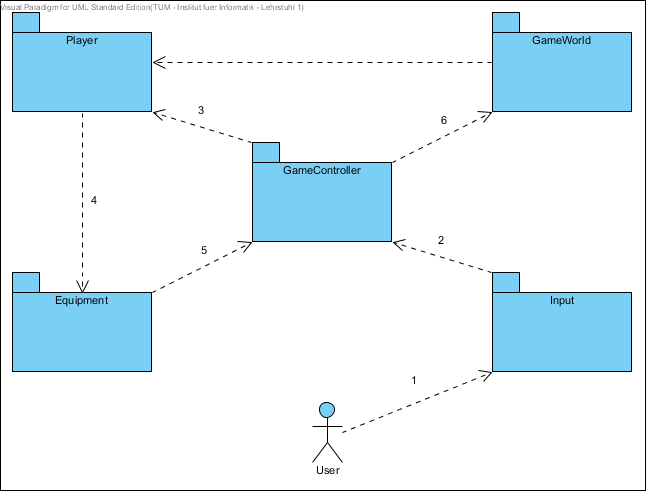
\includegraphics[width=1.0\textwidth]{images/global_control_flow}
\caption[UML-Paketdiagramm: Globaler Kontrollfluss]{UML-Paketdiagramm: Globaler Kontrollfluss}
\label{figure:global_control_flow}
\end{figure}

\section{Globaler Kontrollfluss}
\label{section:GlobalControlFlow}
Der f�r Computerspiele typische Kontrollfluss geht vom Spieler aus, der mit seinen Eingaben Ereignisse ausl�st.
Beispielsweise k�nnte der Spieler eine Taste dr�cken mit dem Ziel, einen Cube (mithilfe des Pick'n'Place-Equipments) in
der Spielwelt zu platzieren. Der Tastendruck wird vom Paket Input detektiert und in einen Steuerbefehl umgesetzt (z.B.
"`benutze equipment"'), welcher dann an das GameController-Paket weitergereicht wird. Dieses ermittelt die daraus
resultierende Reaktion, n�mlich dem Player-Paket den Befehl zu geben, das aktuelle Equipment des Spielers zu ermitteln
und dessen Benutzung anzusto�en, wodurch der Befehl im Equipment-Paket landet. Dort ist die auszuf�hrende Aktion f�r das
Pick'n'Place-Equipment implementiert (R�ckmeldungen f�r den Spieler, Manipulation der Spielwelt usw.).
Das Equipment-Paket meldet folglich dem GameController-Paket die gew�nschte Manipulation der Spielwelt, n�mlich das
Platzieren des im Equipment vorr�tigen Cubes an einer bestimmten Position. Letzendlich wird die Platzierung des Cubes im
Paket GameWorld ausgef�hrt und der Spieler kann den neuen Cube sehen. Dieser beispielhafte Ablauf kann auch anhand der
Nummerierung in Abbildung \ref{figure:global_control_flow} nachvollzogen werden.\\

Das Spiel hat jedoch auch Komponenten, die nicht ereignisgesteuert arbeiten. Das Rendern der virtuellen Welt sowie
deren physikalische Simulation laufen prozedural ab. In einer endlosen Schleife wird mehrmals pro Sekunde ein kleiner
Schritt des physikalischen Modells berechnet und ein neues Bild erzeugt.

\section{Hardware-Software Mapping}
Cydonia ist als Multiplayer-Spiel so konzipiert, dass mehrere Spieler zusammen in einer virtuellen Umgebung spielen.
Dabei nutzt jeder Spieler seinen eigenen Personal Computer (PC) (wie bei einem Singleplayer-Spiel) und die virtuelle
Welt wird zwischen den einzelnen Computern synchronisiert, damit alle Spieler den Lauf der Dinge konsistent erleben.
Dazu ist ein sog. Server n�tig, eine Instanz des Spiels, die die Autorit�t �ber die Geschehnisse in der virtuellen Welt
besitzt, da sonst durch geringf�gige Abweichungen in der Berechnung enorme Unterschiede zwischen den Simulationen auf
den einzelnen Computern entstehen k�nnen. Dieser Server kann bei ausreichender Rechenleistung auch auf einem der PCs der
Spieler laufen, der Einfachkeit halber soll im Folgenden jedoch nur der Fall eines dedizierten Servers betrachtet
werden. Abbildung \ref{figure:hardware_mapping} veranschaulicht die Verteilung der Software-Komponenten auf die
Hardware-Knoten.

\begin{figure}[htbp]
\centering
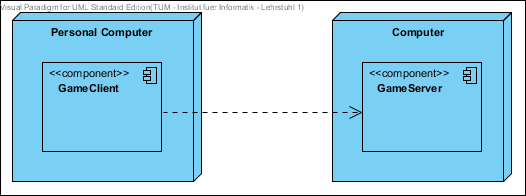
\includegraphics[width=0.8\textwidth]{images/hardware_mapping}
\caption[UML-Verteilungsdiagramm: Beziehung zwischen Software-Komponenten und Hardware-Knoten]{UML-Verteilungsdiagramm: Beziehung zwischen Software-Komponenten und Hardware-Knoten}
\label{figure:hardware_mapping}
\end{figure}



%
%% ---------------------------------------------------------------------------
%%
%% Analyse und Design
%%
%%% ---------------------------------------------------------------------------
%\part[Technische Umsetzung]{Technische Umsetzung}
%\label{part:technicalRealisation}
\chapter{Object Design}
\label{chapter:ObjectDesign}

\section{Dynamisches Modell}

Das dynamische Modell beschreibt die Interaktionen zwischen den Entit�ten des statischen Modells.

\subsection{Neuer Spieler tritt bei}
Wenn eine neuer Spieler dem Spiel beitritt, muss er sich zun�chst beim Server melden. Dieser erstellt ein neues
Spieler-Objekt und informiert die bereits vorhandenen Client-Instanzen �ber den Beitritt und die Daten des neuen
Spielers.

\begin{figure}[h]
\centering
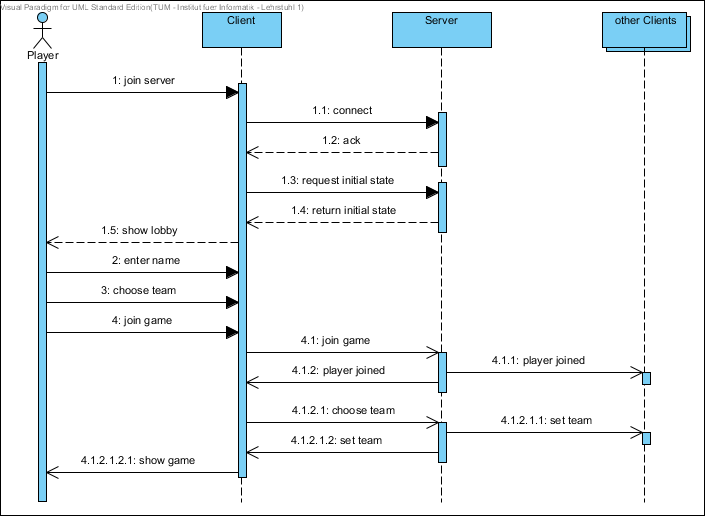
\includegraphics[width=1.0\textwidth]{images/sequence_player_joins}
\caption[Sequenzdiagramm "`Beitritt eines Spielers"']{Sequenzdiagramm "`Beitritt eines Spielers"'}
\label{sequence_player_joins}
\end{figure}


\subsection{Status�berg�nge im System}
Der Client, also die Spiel-Instanz des Spielers, durchl�uft verschiedene Zust�nde. Um alle n�tigen Zust�nde abzubilden
wurden zwei Statusvariablen implementiert: ClientState und GameState. Clientstate stellt den Zustand der Anwendung dar.
M�gliche Werte sind loading, lobby, menu und game. GameState bildet die m�glichen Zust�nde des Spiels ab: down, running,
spectate, roundover. Abbildung \ref{figure:state_machine} zeigt den Zusammenhang der Zust�nde als
Zustands-�bergangs-Diagramm.

\begin{figure}[h]
\centering
\includegraphics[width=1.0\textwidth]{images/state_machine}
\caption[Zustands-�bergangs-Diagramm]{Zustands-�bergangs-Diagramm}
\label{state_machine}
\end{figure}
\section{Einsatz von Entwurfsmustern}

\begin{quotation}
"`Entwurfsmuster sind L�sungswissen f�r allgemeine bzw. immer wiederkehrende Probleme [\ldots]. Ein Entwurfsmuster
besteht aus wenigen Klassen, die durch den Einsatz von Delegation und Vererbung eine robuste und modifizierbare L�sung
erm�glichen."' \cite[S. 719]{Bruegge_2004}
\end{quotation}

In Folgenden werden einige Komponenten von Cydonia vorgestellt und es wird erl�utert, wie bei ihrer Entwicklung
Entwurfsmuster zum Einsatz kommen.


\subsection{Equipment-Erzeugung mittels Abstrakte-Fabrik-Muster}
Da die Equipments der Spieler unterschiedlich sein k�nnen und auch in der Zukunft erweiterbar sein sollen, werden sie
von einer Fabrik-Klasse erzeugt. Die Equipments m�ssen in Client und Server jedoch unterschiedliche Implementierungen
haben. Im Client soll das Equipment grafisch dargestellt und Sounds abgespielt werden. Im Server dagegen sollen
stattdessen die Auswirkungen der Benutzung berechnet werden. Daher kommt hier das Abstrakte-Fabrik-Muster zum Einsatz.
"`Das Abstrakte-Fabrik-Muster setzt Spezifikationsvererbung ein, um die Schnittstelle eines Produkts von seiner
Implementierung zu entkoppeln."'\cite[S. 360]{Bruegge_2004} Um sicherzustellen, dass auf jeder Plattform stets nur die
richtigen Objekte erzeugt werden, also eine konsistente Menge von Objekten vorhanden ist, d�rfen Objekte nur �ber eine
Fabrik erzeugt werden.\cite[S. 360]{Bruegge_2004} Im Fall der Equipments existieren eine ClientEquipmentFactory und eine
ServerEquipmentFactory, die jeweils die von AbstractEquipmentFactory geerbten Methoden zur Erzeugung von Pick'n'Place-
und Swapper-Equipments implementieren. Abbildung \ref{figure:equipment_factory} zeigt die Struktur als
UML-Klassendiagramm.

\begin{figure}[htbp]
\centering
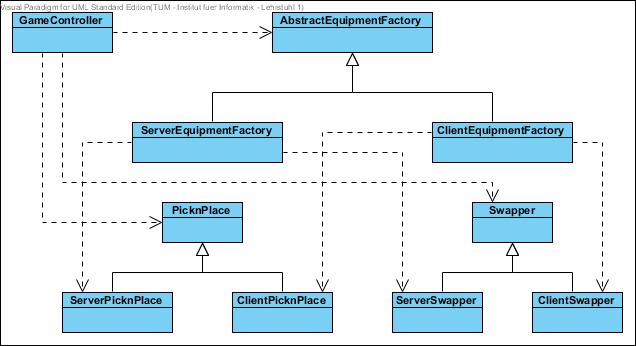
\includegraphics[width=1.0\textwidth]{images/equipment_factory}
\caption[UML-Klassendiagramm: Equipment-Factory]{UML-Klassendiagramm: Equipment-Factory}
\label{figure:equipment_factory}
\end{figure}


\subsection{Szenen-Graph-Erstellung mithilfe des Kompositionsmusters}
\label{subsection:SceneGraph_CompositePattern}
Das Kompositionsmuster ist eine L�sung, um eine Hierarchie beliebiger Breite und Tiefe zu repr�sentieren, sodass sowohl
einzelne Objekte als auch Kompositionen von Objekten durch eine gemeinsame Schnittstelle einheitlich behandelt werden
k�nnen.\cite[S. 724]{Bruegge_2004} Abbildung \ref{figure:composition_spatial} zeigt die Nutzung des Kompositionsmusters
zur Implementierung des Szenen-Graphen in der jMonkeyEngine3. Die Komponente hei�t hier Spatial. Geometry, die
Blatt-Klasse, stellt ein tats�chliches Objekt in der virtuellen Welt dar, definiert durch Formen und Materialien. Das
Kompositum ist Node, welches wiederum andere Spatials als Kindelemente enthalten kann.\par

\begin{figure}[htbp]
\centering
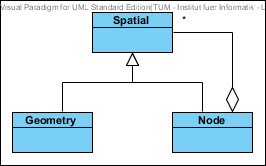
\includegraphics[width=0.6\textwidth]{images/composition_spatial}
\caption[UML-Klassendiagramm: Implementierung Szenen-Graph der jME3]{UML-Klassendiagramm: Implementierung des Szenen-Graph der jME3 unter Verwendung des Kompositionsmusters}
\label{figure:composition_spatial}
\end{figure}

Ein Beispiel f�r die Zusammensetzung der virtuellen Welt aus Spatials kann anhand des Avatars eines Spielers gegeben
werden. Abbildung \ref{figure:composition_avatar} veranschaulicht die Struktur der Spielfigur. Der Wurzelknoten hat drei
Kind\-ele\-men\-te: Kopf, Oberk�rper, Unterk�rper. Der Kopf ist vom Typ Geometry, w�hrend Ober- und Unterk�rper Nodes sind,
die wiederum Kindelemente besitzen, n�mlich Arme, Beine und Torso. Die Unterteilung k�nnte nat�rlich auch noch weiter
gehen: Ein Arm k�nnte zum Beispiel wiederum ein Knoten sein, der aus Oberarm, Unterarm und Hand besteht, wobei die Hand
ebenfalls aus einzelnen Fingern bestehen k�nnte usw. Beliebig feingliedrige Strukturen sind m�glich, je nach gew�nschtem
Detailgrad der Modelle.

\begin{figure}[htbp]
\centering
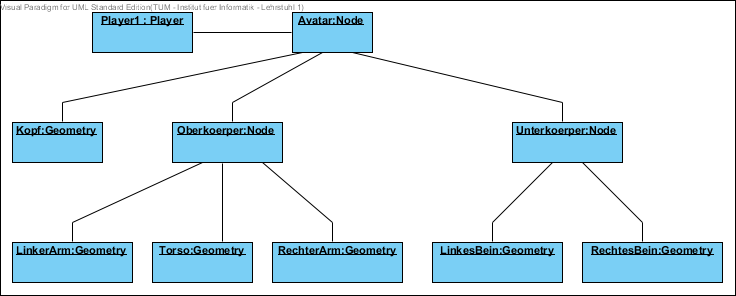
\includegraphics[width=1.0\textwidth]{images/composition_avatar}
\caption[UML-Objektdiagramm: Aufbau des Spieler-Modells]{UML-Objektdiagramm: Aufbau des Spieler-Modells}
\label{figure:composition_avatar}
\end{figure}


\subsection{Event-System mit Beobachtermuster}
Viele Prozesse in Cydonia werden vom Auftreten eines bestimmten Ereignisses angesto�en. Um diese Ereignisse zu
verteilen, gibt es eine zentrale Ereignis-Maschine, die das Beobachtermuster implementiert.\cite[S. 726]{Bruegge_2004}
Objekte, die �ber das Auftreten neuer Ereignisse informiert werden wollen, registrieren sich als Beobachter bei der
Ereignis-Maschine. Au�erdem stellt sie eine Methode zum Ausl�sen von Ereignissen in Form von Objekten des Typs Event
(oder eines Subtyps) zur Verf�gung. Die Ereignisse werden an jeden Beobachter in einem eigenen Thread weitergereicht,
sodass die Bearbeitung parallel stattfinden kann und eine aufw�ndigere Bearbeitung nicht die Weiterleitung des
Ereignisses an andere Beobachter verz�gert. Abbildung \ref{figure:event_system} stellt das Ereignis-System als
UML-Klassendiagramm dar.

\begin{figure}[htbp]
\centering
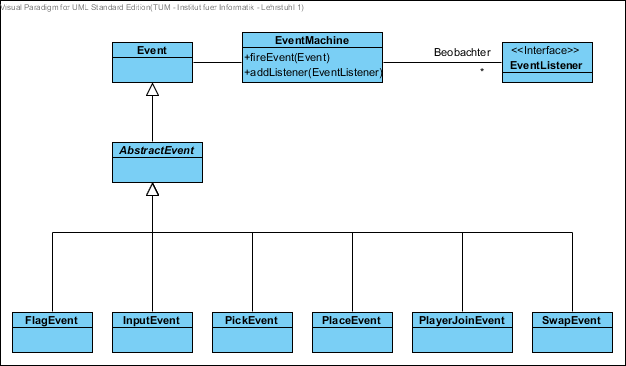
\includegraphics[width=0.8\textwidth]{images/event_system}
\caption[UML-Klassendiagramm: Das Ereignis-System]{UML-Klassendiagramm: Das Ereignis-System}
\label{figure:event_system}
\end{figure}


\subsection{Zustandsabh�ngige Logik mittels Zustandsmuster}
Die Client-Instanz des Spiels steuert gewisse Abl�ufe in Abh�ngigkeit ihres aktuellen Zustands. Zum Beispiel d�rfen
Mausbewegungen und -klicks nicht in Bewegungen und Aktionen des Avatars umgesetzt werden, solange das Men� offen ist, da
der Spieler sonst unkontrollierte Handlungen in der Spielwelt vollzieht. Um zu verhindern, dass zustandsabh�ngige Logik
�ber den gesamten Programmcode verteilt implementiert wird, kommt das Zustandsmuster zum Einsatz. "`Ziel des
Zustandsmusters ist es, die zustandsabh�ngige Logik auf Klassen zu verteilen, die den jeweiligen Zustand des Systems
repr�sentieren."'\cite[229]{Metsker_2006} Vereinfacht dargestellt kann das Spiel zwei Zust�nde ("`Running"' oder "`Menu"')
haben, die sich in der Reaktion auf Benutzereingaben und den dargestellten Interfaces (Men�, HUD, Nachrichten, etc.)
unterscheiden. Abbildung \ref{figure:states_simple} zeigt die Verwendung des Zustandsmusters in Cydonia in Form eines
UML-Klassendiagramms.

\begin{figure}[htbp]
\centering
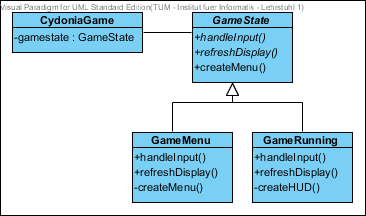
\includegraphics[width=1.0\textwidth]{images/states_simple}
\caption[UML-Klassendiagramm: Zust�nde des Spiels]{UML-Klassendiagramm: Zust�nde des Spiels}
\label{figure:states_simple}
\end{figure}
\section{Details der Implementierung}


\subsection{Dynamisches Modell}

Das dynamische Modell beschreibt die Interaktionen zwischen den Entit�ten des statischen Modells.

\subsubsection{Neuer Spieler tritt bei}
Wenn ein neuer Spieler dem Spiel beitritt, muss er sich zun�chst beim Server melden. Dieser erstellt ein neues
Spieler-Objekt und informiert die bereits vorhandenen Client-Instanzen �ber den Beitritt und die Daten des neuen
Spielers.

\begin{figure}[h]
\centering
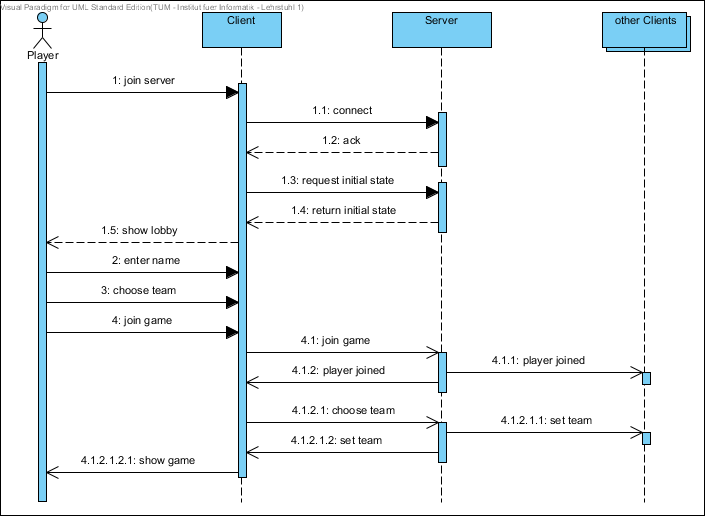
\includegraphics[width=1.0\textwidth]{images/sequence_player_joins}
\caption[UML-Sequenzdiagramm: Beitritt eines Spielers]{UML-Sequenzdiagramm: Beitritt eines Spielers}
\label{sequence_player_joins}
\end{figure}



\subsection{Netzcode}
\label{subsubsection:Netcode}

Um den Spielablauf interaktiv zwischen den Mitspielern zu gestalten, ist es n�tig, die simulierte virtuelle Welt zwischen
dem Server und den einzelnen Client-Instanzen zu synchronisieren. Dies �bernimmt der sog. Netzcode.

Die wichtigsten Aufgaben des Netzcodes sind:
\begin{itemize} 
\item �bertragen von Benutzereingaben in Form von Steuerbefehlen zum Server.
\item Benachrichtigung der Clients �ber Ereignisse, die die simulierte Welt beeinflussen.
\item Senden von Updates �ber den aktuellen Bewegungszustand / die aktuelle Position dynamischer Objekte zum Client.
\end{itemize}

Der Netzcode eines Computerspiels hat f�r die Entwickler teils einen so hohen Stellenwert, dass ein kleineres Spiel
ausschlie�lich als Testplattform f�r den Netzcode eines gro�en Spiels geschrieben wird. So entstand zum Beispiel Mythos
im Rahmen der Entwicklung von Hellgate: London beim Entwickler Flagship Studios \cite{Inerle_2011}.\\

Cydonia verwendet die SpiderMonkey-Bibliothek, mit deren Hilfe Nachrichten �ber das Netzwerk ausgetauscht werden k�nnen
(vgl. dazu \ref{subsubsection:SpiderMonkey}). Dr�ckt zum Beispiel ein Spieler die Taste "`w"', ermittelt das
Input-Mapping den Steuerbefehl "`move forward"'. Daraus wird eine InputMessage erstellt, die die ID des Spielers, den
Befehl "`move forward"' sowie einen Parameter, der das Dr�cken (im Gegensatz zum Loslassen) der Taste kennzeichnet,
enth�lt. Diese Nachricht wird an den Server geschickt. Der Server verarbeitet die erhaltene Nachricht im n�chsten Zyklus
und simuliert in den folgenden Zyklen die Vorw�rtsbewegung des Spielers.\\

In regelm��igen Abst�nden (standardm��ig alle 50 ms) generiert der Server einen sog. Snapshot der virtuellen Welt.
Dieser enth�lt die Positionen und Bewegungsrichtungen aller dynamischen Objekte. Eine Nachricht, die den Snapshot
enth�lt, wird an die Clients geschickt, die ihre Simulation entsprechend anpassen, um die neuen Informationen zu
ber�cksichtigen.\\

Bei einer Latenz von 150 ms zwischen Client und Server w�rde der Spieler das visuelle Feedback zu seiner Eingabe
fr�hestens 150 ms sp�ter erhalten. Eine solche Verz�gerung f�hlt sich unnat�rlich an und st�rt den Spielfluss. Deshalb
wird die Benutzereingabe vom Client in gleicher Weise wie vom Server verarbeitet. Der Spieler bewegt sich also direkt
nach seiner Eingabe vorw�rts. Wenn der n�chste Snapshot vom Server ankommt, ergibt sich zwangsl�ufig eine Abweichung
zwischen den Spielerpositionen. Der Client muss die Spielerposition des Servers �bernehmen, da der Server die alleinige
Autorit�t �ber das Spielgeschehen besitzt. Damit der Spieler nicht pl�tzlich zur�ckspringt, wodurch der Spielfluss
wiederum gest�rt und somit nichts gewonnen w�re, passt der Client die Position des Spielers in kleinen Schritten �ber
einen kurzen Zeitraum hinweg an die vom Server vorgegebene Position an. F�r den Spieler sieht es dann so aus, als ob er
einen kurzen Moment etwas langsamer laufen w�rde, wobei diese Ver�nderung kaum wahrnehmbar ist.\\

Diese Ma�nahme wird auch als Input-Prediction bezeichnet. Sie ist nur eine von vielen m�glichen Ma�nahmen zur Vermeidung
von latenzbasierten Problemen. Vor allem bei Spielen im Internet, wo die Latenzzeiten im Vergleich zum lokalen Netzwerk
h�her sind, sind weitere Vorkehrungen n�tig, um einen fehlerfreien Spielfluss zu
gew�hrleisten.\cite{valve_multiplayer}\\

Die Entwickler-Community der Source-Engine des Entwicklers und Publishers Valve hat eine sehr ausf�hrliche und
verst�ndliche Dokumentation der Funktionsweise ihres Netzcodes ver�ffentlicht. Darin finden sich Beschreibungen der
Techniken Entity-Interpolation, Input-Prediction und Lag-Compensation\cite{valve_multiplayer}. Zusammengenommen
erreichen diese Techniken einen deutlich h�heren Wirkungsgrad. Deren Beschreibung sowie Implementierung �bersteigen
jedoch den Rahmen dieser Arbeit.\\

%\section{Details der Implementierung}


\subsection{Dynamisches Modell}

Das dynamische Modell beschreibt die Interaktionen zwischen den Entit�ten des statischen Modells.

\subsubsection{Neuer Spieler tritt bei}
Wenn ein neuer Spieler dem Spiel beitritt, muss er sich zun�chst beim Server melden. Dieser erstellt ein neues
Spieler-Objekt und informiert die bereits vorhandenen Client-Instanzen �ber den Beitritt und die Daten des neuen
Spielers.

\begin{figure}[h]
\centering
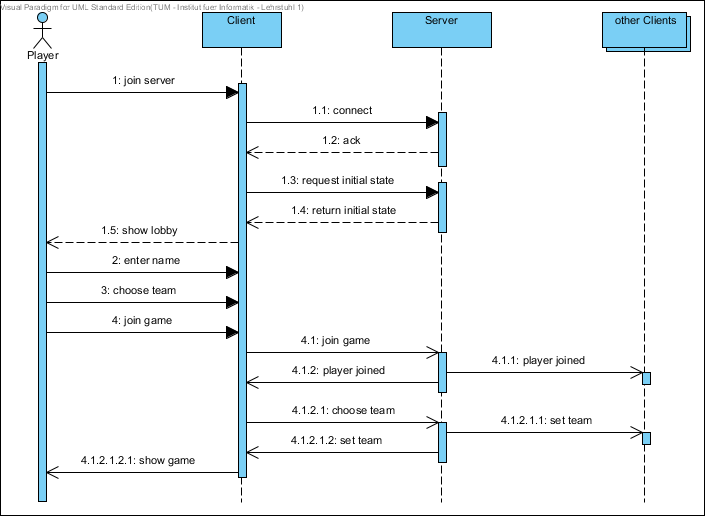
\includegraphics[width=1.0\textwidth]{images/sequence_player_joins}
\caption[UML-Sequenzdiagramm: Beitritt eines Spielers]{UML-Sequenzdiagramm: Beitritt eines Spielers}
\label{sequence_player_joins}
\end{figure}



\subsection{Netzcode}
\label{subsubsection:Netcode}

Um den Spielablauf interaktiv zwischen den Mitspielern zu gestalten, ist es n�tig, die simulierte virtuelle Welt zwischen
dem Server und den einzelnen Client-Instanzen zu synchronisieren. Dies �bernimmt der sog. Netzcode.

Die wichtigsten Aufgaben des Netzcodes sind:
\begin{itemize} 
\item �bertragen von Benutzereingaben in Form von Steuerbefehlen zum Server.
\item Benachrichtigung der Clients �ber Ereignisse, die die simulierte Welt beeinflussen.
\item Senden von Updates �ber den aktuellen Bewegungszustand / die aktuelle Position dynamischer Objekte zum Client.
\end{itemize}

Der Netzcode eines Computerspiels hat f�r die Entwickler teils einen so hohen Stellenwert, dass ein kleineres Spiel
ausschlie�lich als Testplattform f�r den Netzcode eines gro�en Spiels geschrieben wird. So entstand zum Beispiel Mythos
im Rahmen der Entwicklung von Hellgate: London beim Entwickler Flagship Studios \cite{Inerle_2011}.\\

Cydonia verwendet die SpiderMonkey-Bibliothek, mit deren Hilfe Nachrichten �ber das Netzwerk ausgetauscht werden k�nnen
(vgl. dazu \ref{subsubsection:SpiderMonkey}). Dr�ckt zum Beispiel ein Spieler die Taste "`w"', ermittelt das
Input-Mapping den Steuerbefehl "`move forward"'. Daraus wird eine InputMessage erstellt, die die ID des Spielers, den
Befehl "`move forward"' sowie einen Parameter, der das Dr�cken (im Gegensatz zum Loslassen) der Taste kennzeichnet,
enth�lt. Diese Nachricht wird an den Server geschickt. Der Server verarbeitet die erhaltene Nachricht im n�chsten Zyklus
und simuliert in den folgenden Zyklen die Vorw�rtsbewegung des Spielers.\\

In regelm��igen Abst�nden (standardm��ig alle 50 ms) generiert der Server einen sog. Snapshot der virtuellen Welt.
Dieser enth�lt die Positionen und Bewegungsrichtungen aller dynamischen Objekte. Eine Nachricht, die den Snapshot
enth�lt, wird an die Clients geschickt, die ihre Simulation entsprechend anpassen, um die neuen Informationen zu
ber�cksichtigen.\\

Bei einer Latenz von 150 ms zwischen Client und Server w�rde der Spieler das visuelle Feedback zu seiner Eingabe
fr�hestens 150 ms sp�ter erhalten. Eine solche Verz�gerung f�hlt sich unnat�rlich an und st�rt den Spielfluss. Deshalb
wird die Benutzereingabe vom Client in gleicher Weise wie vom Server verarbeitet. Der Spieler bewegt sich also direkt
nach seiner Eingabe vorw�rts. Wenn der n�chste Snapshot vom Server ankommt, ergibt sich zwangsl�ufig eine Abweichung
zwischen den Spielerpositionen. Der Client muss die Spielerposition des Servers �bernehmen, da der Server die alleinige
Autorit�t �ber das Spielgeschehen besitzt. Damit der Spieler nicht pl�tzlich zur�ckspringt, wodurch der Spielfluss
wiederum gest�rt und somit nichts gewonnen w�re, passt der Client die Position des Spielers in kleinen Schritten �ber
einen kurzen Zeitraum hinweg an die vom Server vorgegebene Position an. F�r den Spieler sieht es dann so aus, als ob er
einen kurzen Moment etwas langsamer laufen w�rde, wobei diese Ver�nderung kaum wahrnehmbar ist.\\

Diese Ma�nahme wird auch als Input-Prediction bezeichnet. Sie ist nur eine von vielen m�glichen Ma�nahmen zur Vermeidung
von latenzbasierten Problemen. Vor allem bei Spielen im Internet, wo die Latenzzeiten im Vergleich zum lokalen Netzwerk
h�her sind, sind weitere Vorkehrungen n�tig, um einen fehlerfreien Spielfluss zu
gew�hrleisten.\cite{valve_multiplayer}\\

Die Entwickler-Community der Source-Engine des Entwicklers und Publishers Valve hat eine sehr ausf�hrliche und
verst�ndliche Dokumentation der Funktionsweise ihres Netzcodes ver�ffentlicht. Darin finden sich Beschreibungen der
Techniken Entity-Interpolation, Input-Prediction und Lag-Compensation\cite{valve_multiplayer}. Zusammengenommen
erreichen diese Techniken einen deutlich h�heren Wirkungsgrad. Deren Beschreibung sowie Implementierung �bersteigen
jedoch den Rahmen dieser Arbeit.\\
%\chapter{Testing}
\label{chapter:Testing}


\section{Anwendertests}

Mehrfach w�hrend der Entwicklung wurde das Spiel Testpersonen vorgesetzt. Diese sollten ohne weitere Vorbereitung spielen und ihre Erfahrungen dann mitteilen.
Dabei wurden viele wesentliche Probleme und Schwachstellen aber auch positive und erhaltenswerte Elemente identifiziert. Die wichtigsten davon sollen im folgenden erl�utert werden.

Der im Rahmen dieser Arbeit entwickelte Spiele-Prototyp hatte zu einem fr�hen Entwicklungszeitpunkt folgenden
Spielablauf: Die Spielwelt bestand aus Bauklotz-�hnlichen W�rfeln, die die Spieler beliebig umbauen konnten. Ziel war es
ausgehend von einem Startpunkt als erster einen Zielpunkt zu erreichen. Dazu mussten Treppen, Br�cken und andere
Konstruktionen gebaut werden. Im Test mit mehreren Spielern zeigte sich, dass die M�glichkeit, dem Gegner W�nde in den
Weg zu bauen oder dessen Konstruktionen wieder zu zerlegen, nicht ausreichte um die Spieler zu motivieren. Ein Spieler
�u�erte sich folgenderma�en: "Mir fehlt was, um den anderen abzuknallen." Ebenso bot sich den Spielern kaum Raum,
kooperativ vorzugehen, was sich an der Aussage eines anderen Spielers erkennen l�sst: "Nein, ich wusste nicht, dass wir
im gleichen Team sind".


%% ---------------------------------------------------------------------------
%%
%% Results and Conclusion
%%
%% ---------------------------------------------------------------------------
%\part[Ergebnisse und Ausblick]{Ergebnisse und Ausblick}
%\label{part:resultsAndConclusion}
\chapter{Schluss}
\label{chapter:Conclusion}

\chapter{Testing}
\label{chapter:Testing}


\section{Anwendertests}

Mehrfach w�hrend der Entwicklung wurde das Spiel Testpersonen vorgesetzt. Diese sollten ohne weitere Vorbereitung spielen und ihre Erfahrungen dann mitteilen.
Dabei wurden viele wesentliche Probleme und Schwachstellen aber auch positive und erhaltenswerte Elemente identifiziert. Die wichtigsten davon sollen im folgenden erl�utert werden.

Der im Rahmen dieser Arbeit entwickelte Spiele-Prototyp hatte zu einem fr�hen Entwicklungszeitpunkt folgenden
Spielablauf: Die Spielwelt bestand aus Bauklotz-�hnlichen W�rfeln, die die Spieler beliebig umbauen konnten. Ziel war es
ausgehend von einem Startpunkt als erster einen Zielpunkt zu erreichen. Dazu mussten Treppen, Br�cken und andere
Konstruktionen gebaut werden. Im Test mit mehreren Spielern zeigte sich, dass die M�glichkeit, dem Gegner W�nde in den
Weg zu bauen oder dessen Konstruktionen wieder zu zerlegen, nicht ausreichte um die Spieler zu motivieren. Ein Spieler
�u�erte sich folgenderma�en: "Mir fehlt was, um den anderen abzuknallen." Ebenso bot sich den Spielern kaum Raum,
kooperativ vorzugehen, was sich an der Aussage eines anderen Spielers erkennen l�sst: "Nein, ich wusste nicht, dass wir
im gleichen Team sind".
\chapter{Ergebnisse}
\label{chapter:Results}
\section{Ausblick}

Ist der Versuch, Shooter-Spieler von einem gewaltfreien Spiel zu �berzeugen, gegl�ckt? Diese Frage ist wohl noch nicht
beantwortet. Der Prototyp ist noch nicht ausgereift genug, um es mit anderen Spielen auf dem Markt aufzunehmen. Auch
haben erst eine kleine Auswahl von Spielern die Gelegenheit gehabt, Cydonia zu testen. Doch die ersten Versuche zeigen,
dass es sich lohnt, den eingeschlagenen Weg weiter zu gehen. 

\subsection{Die n�chsten Schritte}
Damit das Konzept von Cydonia Erfolg haben kann, muss aus dem Prototyp ein fertiges Spiel werden. Viele Details wurden
bei der Entwicklung vernachl�ssigt, einfach weil es zu viel Zeit kostet, sich mit ihnen zu befassen. Der Fokus lag auf
der Untersuchung des gewaltfreien Konzepts und seiner Elemente. Passende Avatarmodelle, Equipment-Modelle, Animationen,
Men�s, indivualisierbare Steuerung, detaillierte Ansicht der verf�gbaren Server, In-Game-Chat, Ping-Anzeige um nur ein
paar der Dinge zu nennen, die noch nicht fertig oder garnicht vorhanden sind. Wie in Abschnitt
\ref{subsubsection:Netcode} bereits erw�hnt, ist der Netzcode nur grundlegend implementiert und m�sste starkt optimiert
werden, vor allem wenn Cydonia auch �ber das Internet gespielt werden soll.


%\chapter{Ergebnisse}
\label{chapter:Results}
%\section{Ausblick}

Ist der Versuch, Shooter-Spieler von einem gewaltfreien Spiel zu �berzeugen, gegl�ckt? Diese Frage ist wohl noch nicht
beantwortet. Der Prototyp ist noch nicht ausgereift genug, um es mit anderen Spielen auf dem Markt aufzunehmen. Auch
haben erst eine kleine Auswahl von Spielern die Gelegenheit gehabt, Cydonia zu testen. Doch die ersten Versuche zeigen,
dass es sich lohnt, den eingeschlagenen Weg weiter zu gehen. 

\subsection{Die n�chsten Schritte}
Damit das Konzept von Cydonia Erfolg haben kann, muss aus dem Prototyp ein fertiges Spiel werden. Viele Details wurden
bei der Entwicklung vernachl�ssigt, einfach weil es zu viel Zeit kostet, sich mit ihnen zu befassen. Der Fokus lag auf
der Untersuchung des gewaltfreien Konzepts und seiner Elemente. Passende Avatarmodelle, Equipment-Modelle, Animationen,
Men�s, indivualisierbare Steuerung, detaillierte Ansicht der verf�gbaren Server, In-Game-Chat, Ping-Anzeige um nur ein
paar der Dinge zu nennen, die noch nicht fertig oder garnicht vorhanden sind. Wie in Abschnitt
\ref{subsubsection:Netcode} bereits erw�hnt, ist der Netzcode nur grundlegend implementiert und m�sste starkt optimiert
werden, vor allem wenn Cydonia auch �ber das Internet gespielt werden soll.

 


% ---------------------------------------------------------------------------
%
% Appendix
%
% ---------------------------------------------------------------------------

\part*{Appendix}
\addcontentsline{toc}{part}{Appendix}

\appendix %---------------------------------------

\chapter{Anwendungsf�lle}
\label{chapter:UseCaseDescriptions}

\section{Bewegen}
\begin{tabular}{|p{3cm}|p{9cm}|}
    \hline
	\textbf{Anwendungs-fallname} & Bewegen \\ \hline
	\textbf{Akteure} & Initialisiert von Spieler \\ \hline
	\multirow{7}{*}{\textbf{Ereignisfluss}} & 1) Der Spieler m�chte sich in der virtuellen Welt bewegen. Dazu visiert er sein Ziel an. \\[0.1cm]
	 & 2) Der Spieler kann vorw�rts oder r�ckw�rts gehen, seitw�rts gehen, seine Blickrichtung �ndern oder springen. \\[0.1cm]
	 & \leftskip=1cm 3) Die Position und Blickrichtung des Spielers in der Welt �ndert sich entsprechend. \\ \hline
	\textbf{Anfangs-bedingungen} &  \\ \hline
	\textbf{Abschluss-bedingungen} &  \\ \hline
	\textbf{Qualit�ts-anforderungen} & St��t der Spieler an Hindernisse, muss die Bewegung gestoppt werden. \newline Die Steuerbefehle m�ssen gleichzeitig verwendbar sein. \\ \hline
\end{tabular}


\section{Equipment Wechseln}
\begin{tabular}{|p{3cm}|p{9cm}|}
    \hline
	\textbf{Anwendungs-fallname} & Epuipment wechseln \\ \hline
	\textbf{Akteure} & Initialisiert von Spieler \\ \hline
	\multirow{7}{*}{\textbf{Ereignisfluss}} & 1) Der Spieler m�chte ein anderes Equipment benutzen. Dazu wechselt er zu dem neuen Equipment. \\[0.1cm]
	 & \leftskip=1cm 2) Das bisherige Equipment wird deaktiviert, das neue Equipment aktiviert. der Spieler bekommt eine visuelle R�ckmeldung �ber den Wechsel. \\ \hline
	\textbf{Anfangs-bedingungen} & Der Spieler muss mehrere Equipments zur Verf�gung haben. \\ \hline
	\textbf{Abschluss-bedingungen} & Das neue Equipment muss aktiv und benutzbar sein. \\ \hline
	\textbf{Qualit�ts-anforderungen} & Alle Equipments m�ssen beim Wechsel ihren Zustand bewahren. \\ \hline
\end{tabular}


\newpage
\section{Cube bewegen}
\begin{tabular}{|p{3cm}|p{9cm}|}
    \hline
	\textbf{Anwendungs-fallname} & Cube bewegen \\ \hline
	\textbf{Akteure} & Initialisiert von Spieler \\ \hline
	\multirow{7}{*}{\textbf{Ereignisfluss}} & 1) Der Spieler m�chte einen Cube bewegen. Dazu visiert er den Cube an. \\[0.1cm]
	 & 2) Der Spieler benutzt die Funktion "`Aufnehmen"' des Equipments um den Cube aufzunehmen. \\[0.1cm]
	 & \leftskip=1cm 3) Der Cube wird aus der Spielwelt entfernt und erscheint im Inventar des Equipments. \\[0.1cm]
	 & 4) Der Spieler kann sich nun beliebig bewegen (siehe Anwendungsfall "`Bewegen"'). \\[0.1cm]
	 & 5) Der Spieler visiert die Stelle an, an der er den Cube platzieren m�chte. \\[0.1cm]
	 & 6) Der Spieler benutzt die Funktion "`Platzieren"' des Equipments um den Cube zu platzieren. \\[0.1cm]
	 & \leftskip=1cm 7) Der Cube verschwindet aus dem Inventar des Equipments und wird in die Spielwelt eingef�gt. \\ \hline
	\textbf{Anfangs-bedingungen} & Ein beweglicher Cube muss in Sichtweite des Spielers in der Spielwelt vorhanden sein.\newline Der Spieler muss das Pick'n'Place-Equipment ausgew�hlt haben. \newline Das Pick'n'Place-Equipment muss zur Aufnahme eines Cubes bereit sein. \\ \hline
	\textbf{Abschluss-bedingungen} & Der Cube muss in der Welt vorhanden sein. \newline Das Pick'n'Place-Equipment muss zur erneuten Aufnahme eines Cubes bereit sein. \\ \hline
	\textbf{Qualit�ts-anforderungen} & Unterbricht der Spieler die Aktion zwischen Schritt 3 und Schritt 6, muss der Cube im Inventar erhalten bleiben, bis der Spieler die Aktion fortsetzt. \\ \hline
\end{tabular}

\newpage
\section{Gegnerische Flagge nehmen}
\begin{tabular}{|p{3cm}|p{9cm}|}
    \hline
	\textbf{Anwendungs-fallname} & Flagge nehmen \\ \hline
	\textbf{Akteure} & Initialisiert von Spieler \\ \hline
	\multirow{7}{*}{\textbf{Ereignisfluss}} & 1) Der Spieler m�chte die gegnerische Flagge aufnehmen. Dazu bewegt er sich zu der Flagge (siehe Anwendungsfall "`Bewegen"'). \\[0.1cm]
	 & \leftskip=1cm 2) Wenn der Spieler die Flagge ber�hrt, nimmt er sie auf. Der Spieler bekommt angezeigt, dass er die Flagge bei sich tr�gt. \\[0.1cm]
	 & 3) Der Spieler kann sich nun beliebig bewegen (siehe Anwendungsfall "`Bewegen"'). \\[0.1cm]
	 & \leftskip=1cm 4) Die Flagge bewegt sich mit dem Spieler mit. \\ \hline
	\textbf{Anfangs-bedingungen} & Kein Spieler darf die gegnerische Flagge bei sich tragen.\newline Die gegnerische Flagge muss f�r der Spieler erreichbar sein. \\ \hline
	\textbf{Abschluss-bedingungen} & Die Flagge muss sich mit dem Spieler bewegen. \\ \hline
	\textbf{Qualit�ts-anforderungen} & Der Status der Flagge muss dem Spieler zu jeder Zeit angezeigt werden. \\ \hline
\end{tabular}

\newpage
\section{Gegnerische Flagge erobern}
\begin{tabular}{|p{3cm}|p{9cm}|}
    \hline
	\textbf{Anwendungs-fallname} & Einen Punkt erzielen \\ \hline
	\textbf{Akteure} & Initialisiert von Spieler \\ \hline
	\multirow{7}{*}{\textbf{Ereignisfluss}} & 1) Der Spieler m�chte die gegnerische Flagge erobern. Dazu bewegt sich zu seiner Flagge in seiner Basis (siehe Anwendungsfall "`Bewegen"'). \\[0.1cm]
	 & \leftskip=1cm 2) Ist die Flagge des Spielers in seiner Basis, erh�lt sein Team einen Punkt und die gegnerische Flagge wird zur�ckgesetzt. \\[0.1cm]
	 & 3) Ist die Flagge des Spielers nicht in seiner Basis, kann der Spieler warten, bis sie wieder da ist, und dann den Punkt erzielen. \\ \hline
	\textbf{Anfangs-bedingungen} & Der Spieler muss die gegnerische Flagge bei sich tragen (siehe Anwendungsfall "`Gegnerische Flagge nehmen"'). \\ \hline
	\textbf{Abschluss-bedingungen} & Die gegnerische Flagge muss sich wieder in ihrer Basis befinden. \\ \hline
	\textbf{Qualit�ts-anforderungen} & Der Status der Flagge muss dem Spieler zu jeder Zeit angezeigt werden. \\ \hline
\end{tabular}


\newpage
\section{Objekte swappen}
\begin{tabular}{|p{3cm}|p{9cm}|}
    \hline
	\textbf{Anwendungs-fallname} & Objekte swappen \\ \hline
	\textbf{Akteure} & Initialisiert von Spieler \\ \hline
	\multirow{7}{*}{\textbf{Ereignisfluss}} & 1) Der Spieler m�chte zwei Objekte swappen. Dazu visiert er ein Ojbekt an. \\[0.1cm]
	 & 2) Der Spieler benutzt das Equipment das Objekt zu markieren. \\[0.1cm]
	 & \leftskip=1cm 3) Die Markierung wird visualisiert, indem das markierte Objekt f�r den Spieler hervorgehoben dargestellt wird. \\[0.1cm]
	 & 4) Der Spieler kann sich nun beliebig bewegen (siehe Anwendungsfall "`Bewegen"'). \\[0.1cm]
	 & 5) Der Spieler visiert ein weiteres Objekt an. \\[0.1cm]
	 & 6) Der Spieler benutzt das Equipment um das Objekt zu markieren. \\[0.1cm]
	 & \leftskip=1cm 7) Die beiden markierten Objekte tauschen ihre Positionen in der Spielwelt. \\[0.1cm]
	 & \leftskip=1cm 8) Wenn eines der Objekte ein gegnerischer Spieler ist und dieser die Flagge bei sich tr�gt, verliert er die Flagge. Sie bleibt an der urspr�nglichen Position des gegnerischen Spielers. \\ \hline
	\textbf{Anfangs-bedingungen} & Zwei Objekte, die der Spieler swappen kann, m�ssen sich in der Spielwelt befinden. \newline Der Spieler muss das Swapper-Equipment ausgew�hlt haben. \\ \hline
	\textbf{Abschluss-bedingungen} & Beide Objekte m�ssen an der jeweils anderen Position in der Spielwelt sein. \newline Die beiden Objekte m�ssen unmarkiert sein. \newline Die beiden Markierungen des Swapper-Equipments m�ssen wieder frei sein. \\ \hline
	\textbf{Qualit�ts-anforderungen} & Setzt der Spieler eine bereits gesetzte Markierung auf ein anderes Objekt, muss die Markierung des urspr�nglichen Objekts aufgehoben werden. \newline Ein Spieler darf die gegnerische Flagge nichtverlieren, wenn er von einem Spieler im \emph{gleichen} Team geswappet wird. \\ \hline
\end{tabular}


\newpage
\section{Eigene Flagge zur�ckholen}
\begin{tabular}{|p{3cm}|p{9cm}|}
    \hline
	\textbf{Anwendungs-fallname} & Eigene Flagge zur�ckholen \\ \hline
	\textbf{Akteure} & Initialisiert von Spieler \\ \hline
	\multirow{7}{*}{\textbf{Ereignisfluss}} & 1) Der Spieler m�chte die Flagge seines Teams zur�ckholen. Dazu bewegt er sich zu der Flagge (siehe Anwendungsfall "`Bewegen"'). \\[0.1cm]
	 & 2) Falls ein gegnerischer Spieler die Flagge bei sich tr�gt, muss der Spieler den gegnerischen Spieler swappen, damit dieser die Flagge verliert (siehe Anwendungsfall "`Objekte swappen"'). \\[0.1cm]
	 & \leftskip=1cm 3) Wenn der Spieler die Flagge ber�hrt, wird die Flagge zur�ckgesetzt. Der Spieler bekommt angezeigt, dass die Flagge wieder in der Basis ist. \\ \hline
	\textbf{Anfangs-bedingungen} & Die Flagge des Spielers darf sich nicht in ihrer Basis befinden. \\ \hline
	\textbf{Abschluss-bedingungen} & Die Flagge des Spielers muss sich in ihrer Basis befinden. \\ \hline
	\textbf{Qualit�ts-anforderungen} & Der Status der Flagge muss dem Spieler zu jeder Zeit angezeigt werden. \\ \hline
\end{tabular}
\chapter{Detailed Descriptions}
\label{chapter:DetailedDescriptions}
Here come the details that are not supposed to be in the regular text.



